%%%%%%%%%%%%%%%%%%%%%%%%%%%%%%%%%%%%%%%%%
% Cleese Assignment (For Students)
% LaTeX Template
% Version 2.0 (27/5/2018)
%
% This template originates from:
% http://www.LaTeXTemplates.com
%
% Author:
% Vel (vel@LaTeXTemplates.com)
%
% License:
% CC BY-NC-SA 3.0 (http://creativecommons.org/licenses/by-nc-sa/3.0/)
% 
%%%%%%%%%%%%%%%%%%%%%%%%%%%%%%%%%%%%%%%%%

%----------------------------------------------------------------------------------------
%	PACKAGES AND OTHER DOCUMENT CONFIGURATIONS
%----------------------------------------------------------------------------------------

\documentclass[11pt]{article}
\usepackage{float}

%\usepackage[printwatermark]{xwatermark}
%\newwatermark[allpages,color=gray!50,angle=45,scale=2.5,xpos=-5,ypos=-5]{Mohammad Hadi}

%%%%%%%%%%%%%%%%%%%%%%%%%%%%%%%%%%%%%%%%%
% Cleese Assignment
% Structure Specification File
% Version 1.0 (27/5/2018)
%
% This template originates from:
% http://www.LaTeXTemplates.com
%
% Author:
% Vel (vel@LaTeXTemplates.com)
%
% License:
% CC BY-NC-SA 3.0 (http://creativecommons.org/licenses/by-nc-sa/3.0/)
% 
%%%%%%%%%%%%%%%%%%%%%%%%%%%%%%%%%%%%%%%%%

%----------------------------------------------------------------------------------------
%	PACKAGES AND OTHER DOCUMENT CONFIGURATIONS
%----------------------------------------------------------------------------------------

\usepackage{lastpage} % Required to determine the last page number for the footer

\usepackage{graphicx} % Required to insert images

\setlength\parindent{0pt} % Removes all indentation from paragraphs

\usepackage[most]{tcolorbox} % Required for boxes that split across pages

\usepackage{booktabs} % Required for better horizontal rules in tables

\usepackage{listings} % Required for insertion of code

\usepackage{etoolbox} % Required for if statements

%----------------------------------------------------------------------------------------
%	MARGINS
%----------------------------------------------------------------------------------------

\usepackage{geometry} % Required for adjusting page dimensions and margins

\geometry{
	paper=a4paper, % Change to letterpaper for US letter
	top=3cm, % Top margin
	bottom=3cm, % Bottom margin
	left=2.5cm, % Left margin
	right=2.5cm, % Right margin
	headheight=14pt, % Header height
	footskip=1.4cm, % Space from the bottom margin to the baseline of the footer
	headsep=1.2cm, % Space from the top margin to the baseline of the header
	%showframe, % Uncomment to show how the type block is set on the page
}

%----------------------------------------------------------------------------------------
%	FONT
%----------------------------------------------------------------------------------------

\usepackage[utf8]{inputenc} % Required for inputting international characters
\usepackage[T1]{fontenc} % Output font encoding for international characters

\usepackage[sfdefault,light]{roboto} % Use the Roboto font

%----------------------------------------------------------------------------------------
%	HEADERS AND FOOTERS
%----------------------------------------------------------------------------------------

\usepackage{fancyhdr} % Required for customising headers and footers

\pagestyle{fancy} % Enable custom headers and footers

\lhead{\small\assignmentClass\ifdef{\assignmentClassInstructor}{\ (\assignmentClassInstructor):}{}\ \assignmentTitle} % Left header; output the instructor in brackets if one was set
\chead{} % Centre header
\rhead{\small\ifdef{\assignmentAuthorName}{\assignmentAuthorName}{\ifdef{\assignmentDueDate}{Due\ \assignmentDueDate}{}}} % Right header; output the author name if one was set, otherwise the due date if that was set

\lfoot{} % Left footer
\cfoot{\small Page\ \thepage\ of\ \pageref{LastPage}} % Centre footer
\rfoot{} % Right footer

\renewcommand\headrulewidth{0.5pt} % Thickness of the header rule

%----------------------------------------------------------------------------------------
%	MODIFY SECTION STYLES
%----------------------------------------------------------------------------------------

\usepackage{titlesec} % Required for modifying sections

%------------------------------------------------
% Section

\titleformat
{\section} % Section type being modified
[block] % Shape type, can be: hang, block, display, runin, leftmargin, rightmargin, drop, wrap, frame
{\Large\bfseries} % Format of the whole section
{\assignmentQuestionName~\thesection} % Format of the section label
{6pt} % Space between the title and label
{} % Code before the label

\titlespacing{\section}{0pt}{0.5\baselineskip}{0.5\baselineskip} % Spacing around section titles, the order is: left, before and after

%------------------------------------------------
% Subsection

\titleformat
{\subsection} % Section type being modified
[block] % Shape type, can be: hang, block, display, runin, leftmargin, rightmargin, drop, wrap, frame
{\itshape} % Format of the whole section
{(\alph{subsection})} % Format of the section label
{4pt} % Space between the title and label
{} % Code before the label

\titlespacing{\subsection}{0pt}{0.5\baselineskip}{0.5\baselineskip} % Spacing around section titles, the order is: left, before and after

\renewcommand\thesubsection{(\alph{subsection})}

%----------------------------------------------------------------------------------------
%	CUSTOM QUESTION COMMANDS/ENVIRONMENTS
%----------------------------------------------------------------------------------------

% Environment to be used for each question in the assignment
\newenvironment{question}{
	\vspace{0.5\baselineskip} % Whitespace before the question
	\section{} % Blank section title (e.g. just Question 2)
	\lfoot{\small\itshape\assignmentQuestionName~\thesection~continued on next page\ldots} % Set the left footer to state the question continues on the next page, this is reset to nothing if it doesn't (below)
}{
	\lfoot{} % Reset the left footer to nothing if the current question does not continue on the next page
}

%------------------------------------------------

% Environment for subquestions, takes 1 argument - the name of the section
\newenvironment{subquestion}[1]{
	\subsection{#1}
}{
}

%------------------------------------------------

% Command to print a question sentence
\newcommand{\questiontext}[1]{
	\textbf{#1}
	\vspace{0.5\baselineskip} % Whitespace afterwards
}

%------------------------------------------------

% Command to print a box that breaks across pages with the question answer
\newcommand{\answer}[1]{
	\begin{tcolorbox}[breakable, enhanced]
		#1
	\end{tcolorbox}
}

%------------------------------------------------

% Command to print a box that breaks across pages with the space for a student to answer
\newcommand{\answerbox}[1]{
	\begin{tcolorbox}[breakable, enhanced]
		\vphantom{L}\vspace{\numexpr #1-1\relax\baselineskip} % \vphantom{L} to provide a typesetting strut with a height for the line, \numexpr to subtract user input by 1 to make it 0-based as this command is
	\end{tcolorbox}
}

%------------------------------------------------

% Command to print an assignment section title to split an assignment into major parts
\newcommand{\assignmentSection}[1]{
	{
		\centering % Centre the section title
		\vspace{2\baselineskip} % Whitespace before the entire section title
		
		\rule{0.8\textwidth}{0.5pt} % Horizontal rule
		
		\vspace{0.75\baselineskip} % Whitespace before the section title
		{\LARGE \MakeUppercase{#1}} % Section title, forced to be uppercase
		
		\rule{0.8\textwidth}{0.5pt} % Horizontal rule
		
		\vspace{\baselineskip} % Whitespace after the entire section title
	}
}

%----------------------------------------------------------------------------------------
%	TITLE PAGE
%----------------------------------------------------------------------------------------

\author{\textbf{\assignmentAuthorName}} % Set the default title page author field
\date{} % Don't use the default title page date field

\title{
	\thispagestyle{empty} % Suppress headers and footers
	\vspace{0.2\textheight} % Whitespace before the title
	\textbf{\assignmentClass:\ \assignmentTitle}\\[-4pt]
	\ifdef{\assignmentDueDate}{{\small Due\ on\ \assignmentDueDate}\\}{} % If a due date is supplied, output it
	\ifdef{\assignmentClassInstructor}{{\large \textit{\assignmentClassInstructor}}}{} % If an instructor is supplied, output it
	\vspace{0.32\textheight} % Whitespace before the author name
}
 % Include the file specifying the document structure and custom commands

%----------------------------------------------------------------------------------------
%	ASSIGNMENT INFORMATION
%----------------------------------------------------------------------------------------

% Required
\newcommand{\assignmentQuestionName}{Experiment} % The word to be used as a prefix to question numbers; example alternatives: Problem, Exercise
\newcommand{\assignmentClass}{Electrical Circuits Lab (Taught by Mohammad Hadi)\\Manual 3 (Due on DDD.,\ mmm.\ dd,\ yyyy)} % Course (Lecturer)\\Assignment (Due date)
\newcommand{\assignmentTitle}{} % Assignment title or name
\newcommand{\assignmentAuthorName}{Sina Hashemi \& M.Mahdi Shokrzade\\402102668 - 402101985} % Student name\\Student number
%----------------------------------------------------------------------------------------

\newcommand{\PicScale}{0.2}

\begin{document}
\textbf{Real circuit elements are approximate physical implementation of ideal circuit elements. In this experiment, you become familiar with the main limitations of the conventional real circuit elements such as resistors, capacitors, and diodes.
}
%----------------------------------------------------------------------------------------
%	TITLE PAGE
%----------------------------------------------------------------------------------------

\assignmentSection{Mandatory Experiments}

%----------------------------------------------------------------------------------------
%	QUESTION 1
%----------------------------------------------------------------------------------------

\begin{question}

    \questiontext{Consider the circuit shown in Fig. \ref{fig:cir1} }

    \begin{figure}[H]
        \centering
        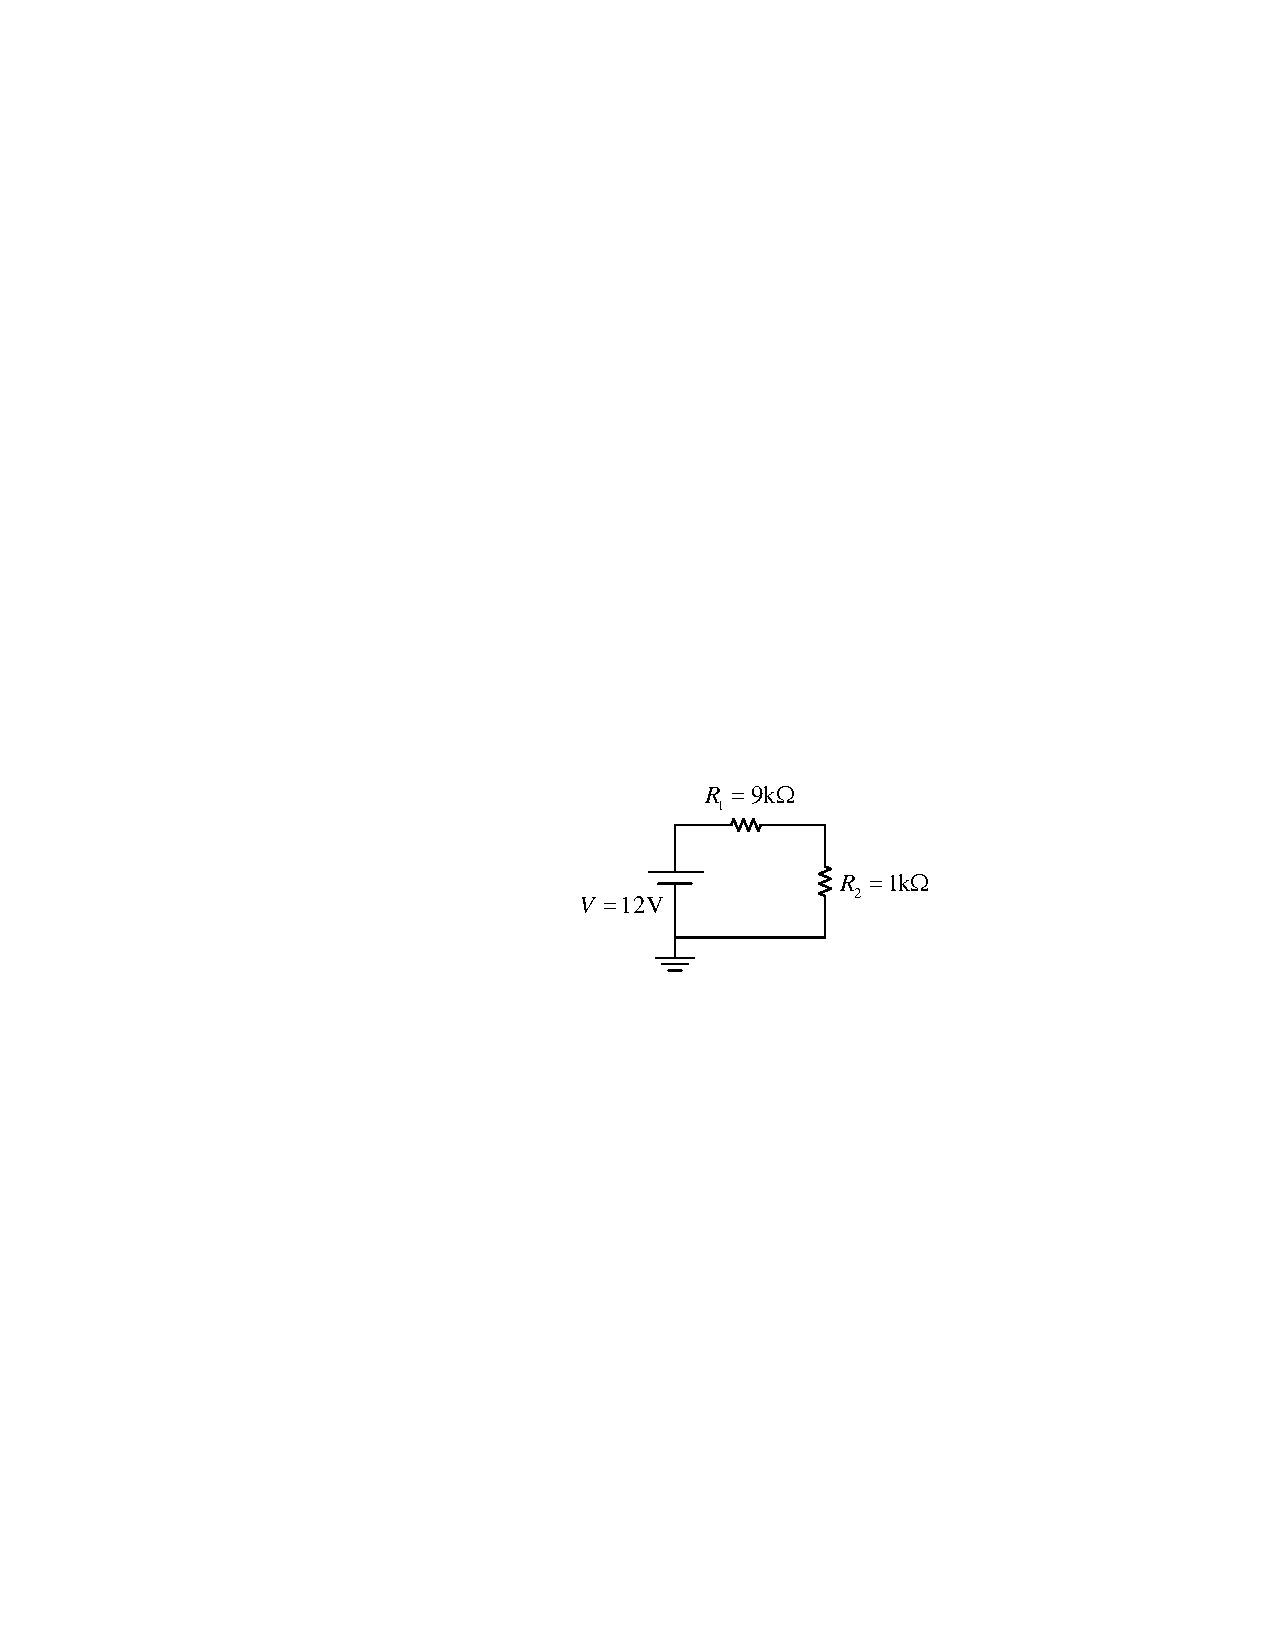
\includegraphics[scale=1.2,angle=0]{Fig/cir1.pdf}
        \caption{A voltage divider circuit.} \label{fig:cir1}
    \end{figure}

    %--------------------------------------------
    \begin{subquestion}{Build the circuit on a breadboard. Can you find a $9$ k$\Omega$ resistor in the stackable element storage box? }
        \answer{
            No because $9k$ is not in E24 standard.
        }
    \end{subquestion}

    %--------------------------------------------
    \begin{subquestion}{Which resistor is a suitable replacement for a $9$ k$\Omega$ resistor? Pick that resistor and read its color code.}
        \answer{
            We used two parallel $18k\Omega$ resistors to obtain $9k\Omega$. We could also use an $8k\Omega$ because E12 resistors have $5\%$ error.
        }
    \end{subquestion}

    %--------------------------------------------
    \begin{subquestion}{Measure the voltage across each resistor. Is there any difference between the measured and analytical values?}
        \answer{
            \begin{figure}[H]
                \centering
                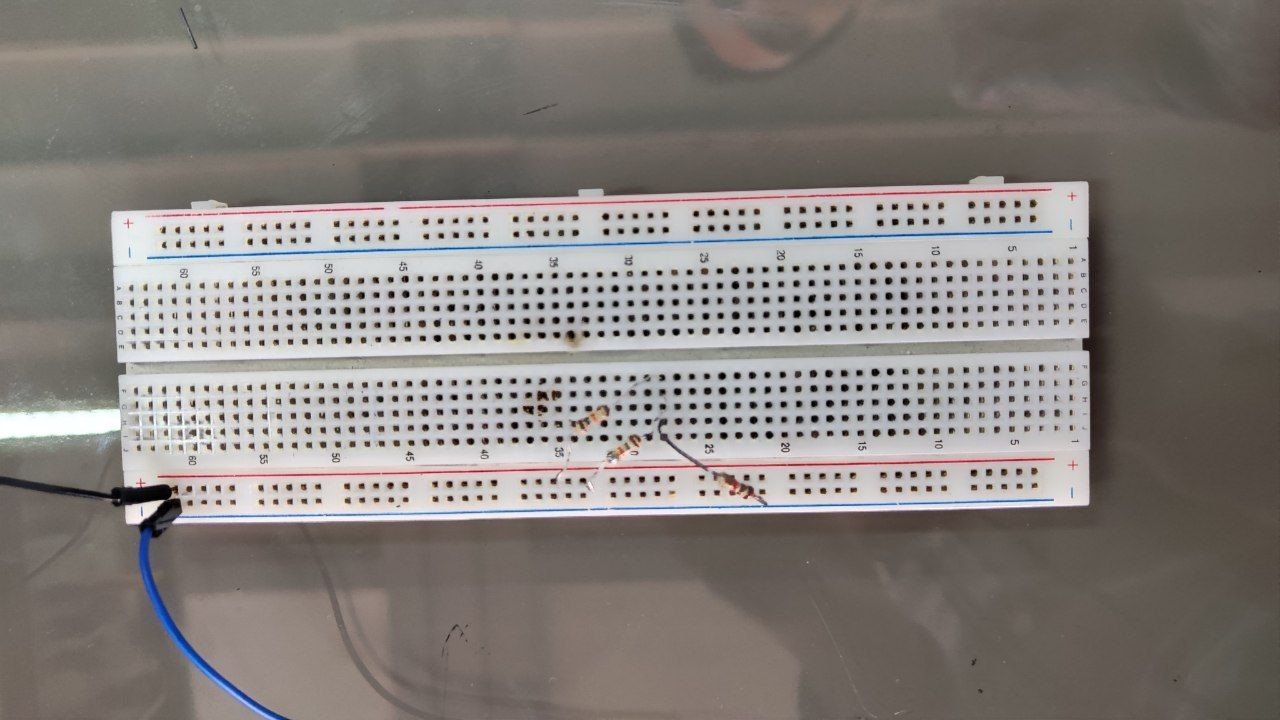
\includegraphics[scale=\PicScale,angle=0]{Fig/1.jpeg}
                \caption{The circuit.}
            \end{figure}
            \begin{figure}[H]
                \centering
                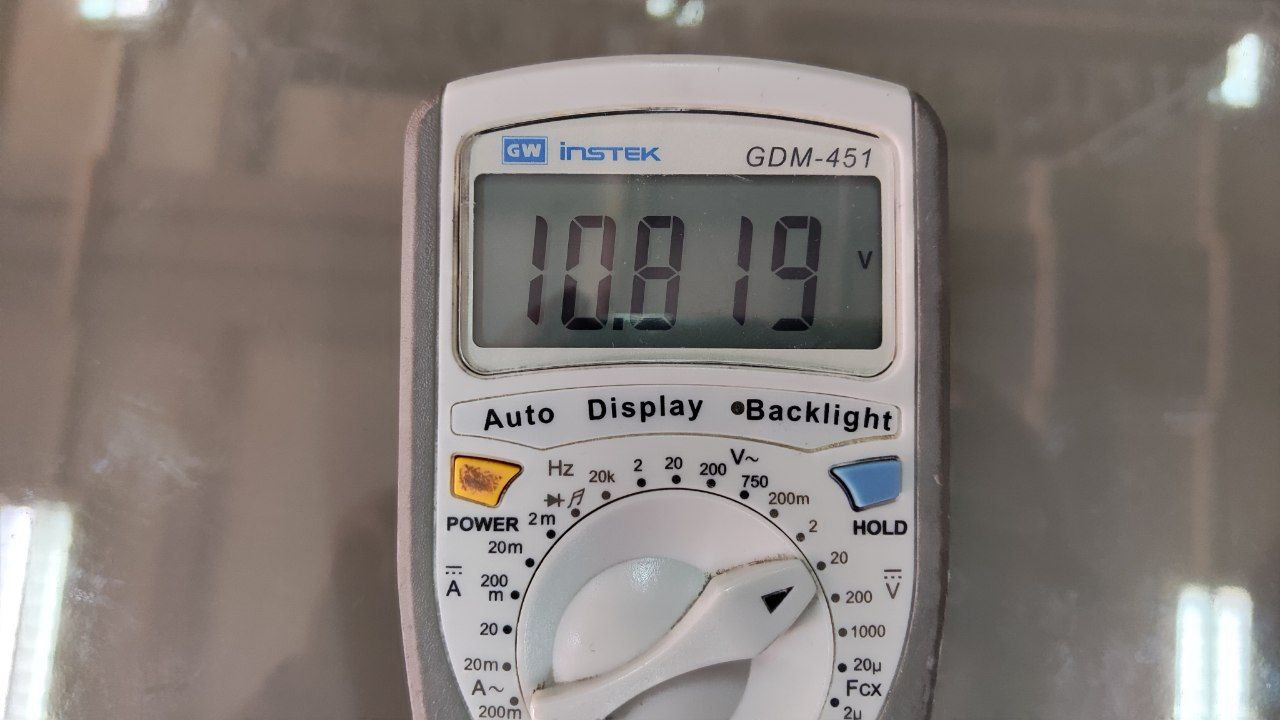
\includegraphics[scale=0.12,angle=0]{Fig/2.jpeg}
                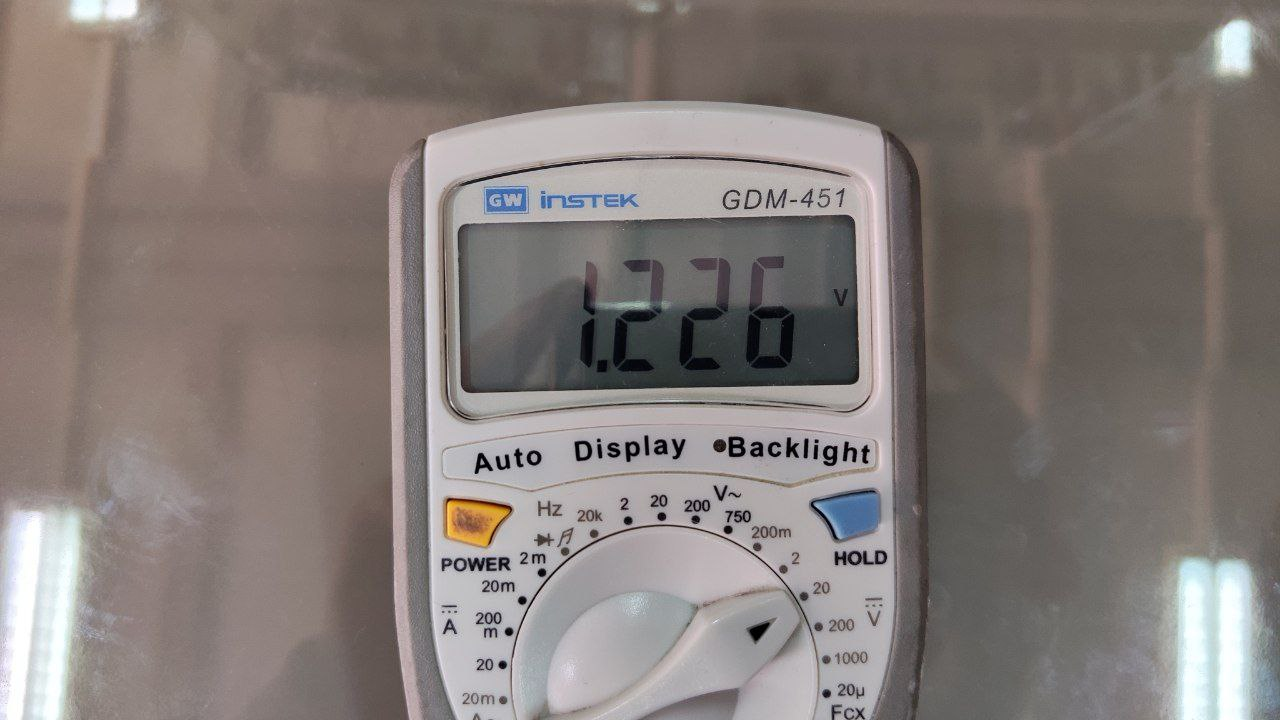
\includegraphics[scale=0.12,angle=0]{Fig/3.jpeg}
                \caption{measured voltage value.}
            \end{figure}
            
        }
    \end{subquestion}

\end{question}


%----------------------------------------------------------------------------------------
%	QUESTION 2
%----------------------------------------------------------------------------------------

\begin{question}

    \questiontext{Each real circuit element has a nominal value within a tolerance band.}

    %--------------------------------------------
    \begin{subquestion}{Pick up ten E12 $1$ k$\Omega$ resistors and measure their resistance. Calculate the maximum, minimum, mean, variance, and standard deviation of the measured values and interpret them considering the nominal and tolerance values. }
        \answer{
            We used E24 resistors instead. \\
            values: $1.0103, 0.9940, 1.0027, 1.0018, 1.0012, 1.0015, 0.9964, 0.9996, 0.9979$ and $1.0135~k\Omega$.
        }
    \end{subquestion}

    %--------------------------------------------
    \begin{subquestion}{Repeat the previous part for ten E12 $10$ $\mu$F capacitors. }
        \answer{
            values: $9.76, 9.64, 9.05, 9.49, 9.19, 9.32, 9.61, 9.73, 9.37$ and $9.31~\mu F$
        }
    \end{subquestion}

\end{question}

%----------------------------------------------------------------------------------------
%	QUESTION 3
%----------------------------------------------------------------------------------------

\begin{question}

    \questiontext{\underline{This experiment should be done by the lab supervisor}. Dependency of the value of a real circuit element on temperature is characterized by a specified temperature coefficient. }

    %--------------------------------------------
    \begin{subquestion}{Measure the resistance of a carbon resistor in room temperature. Redo the measurement when the resistor is heated by a soldering iron and when is cooled by a cooling spray. }
        \answer{}
    \end{subquestion}

    %--------------------------------------------
    \begin{subquestion}{Repeat the previous part for a metal film resistor, a ceramic capacitor, and a multi-layer capacitor. }
        \answer{}
    \end{subquestion}

\end{question}

%----------------------------------------------------------------------------------------
%	QUESTION 4
%----------------------------------------------------------------------------------------

\begin{question}

    \questiontext{\underline{This experiment should be done by the lab supervisor}. Each resistor has a specific maximum power rating. Connect a $0.25$ W $10$ $\Omega$ resistor to a DC power supply using an alligator clip wire. Sweep the voltage from $0$ to $5$ V and observe the results.}

    \answer{}

\end{question}

%----------------------------------------------------------------------------------------
%	QUESTION 4
%----------------------------------------------------------------------------------------

\begin{question}

    \questiontext{\underline{This experiment should be done by the lab supervisor}. Each capacitor has a specific maximum voltage. Further, a capacitor may have a  specific voltage polarity. }

    %--------------------------------------------
    \begin{subquestion}{Connect a $16$ V aluminum electrolytic capacitor directly to a $30$ V DC voltage and observe the results.}
        \answer{
            \begin{figure}[H]
                \centering
                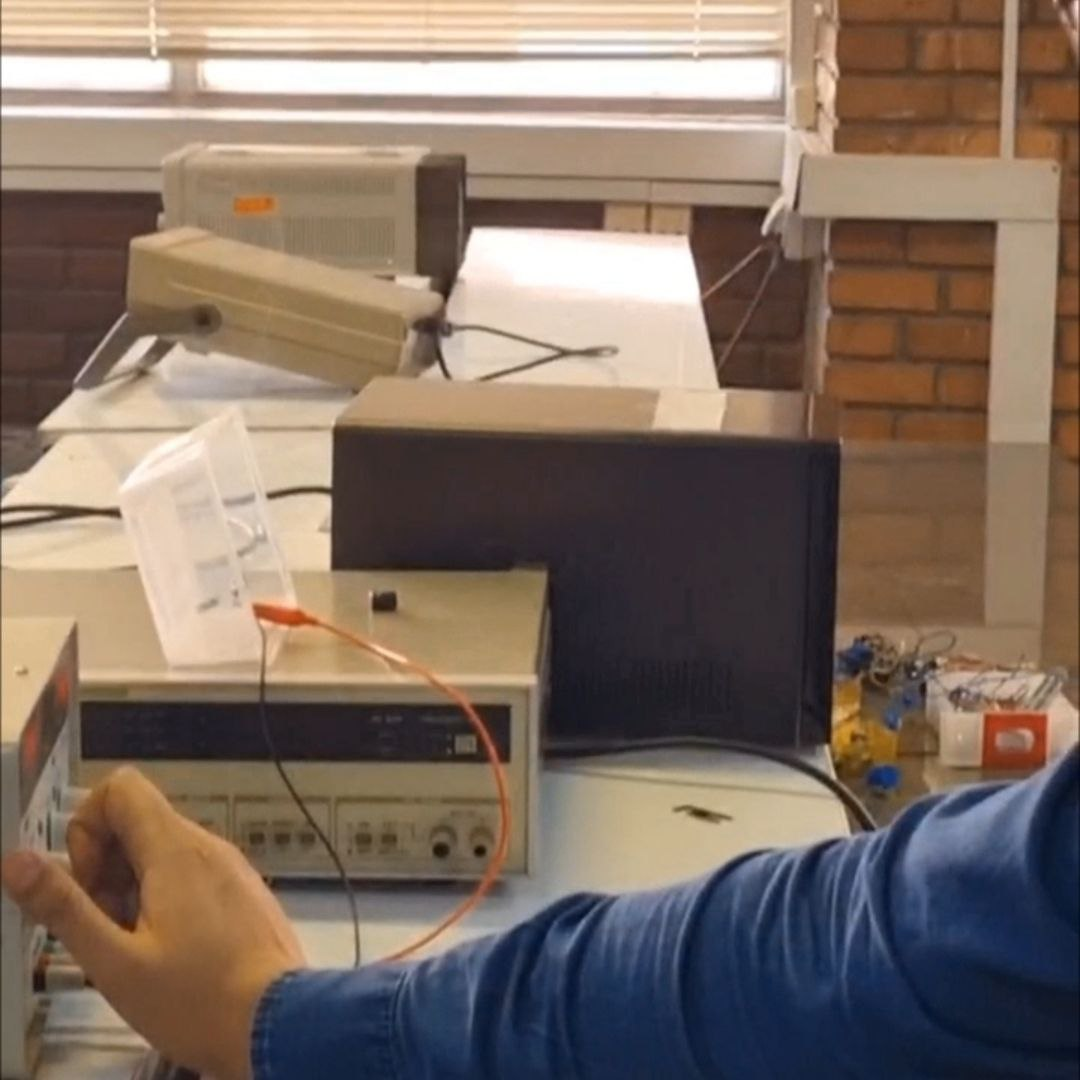
\includegraphics[scale=0.08,angle=0]{Fig/4.jpeg}
                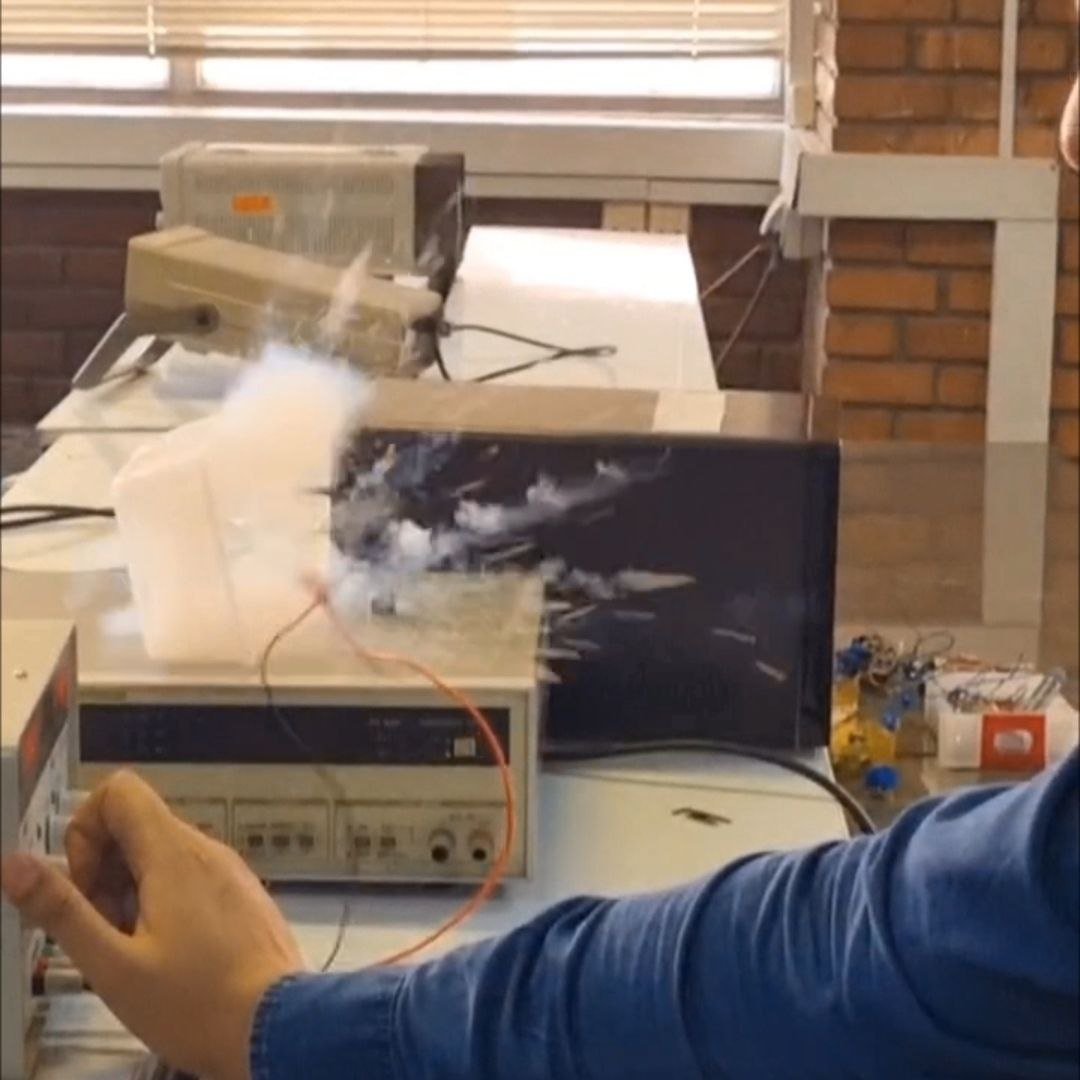
\includegraphics[scale=0.08,angle=0]{Fig/5.jpeg}
                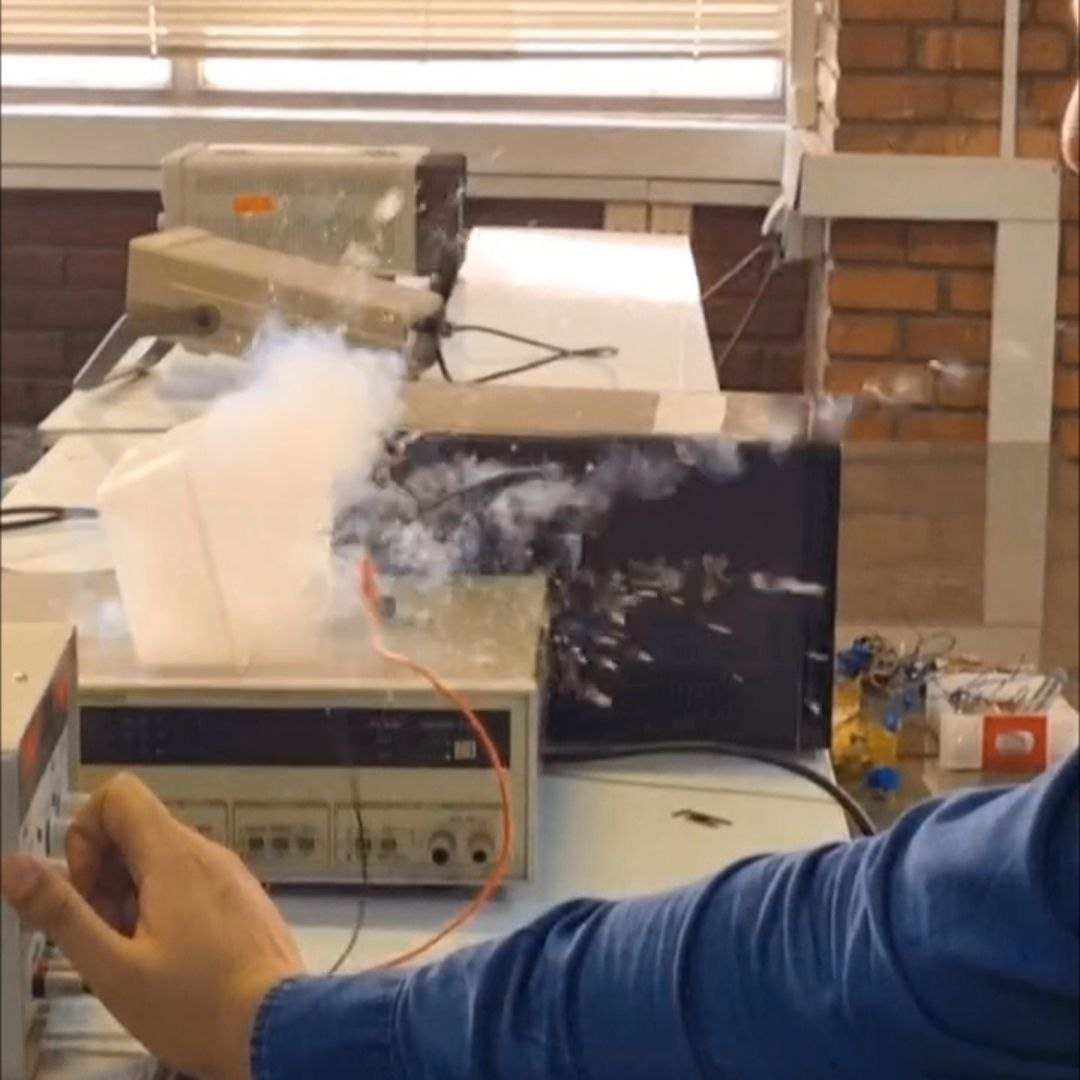
\includegraphics[scale=0.08,angle=0]{Fig/6.jpeg}
                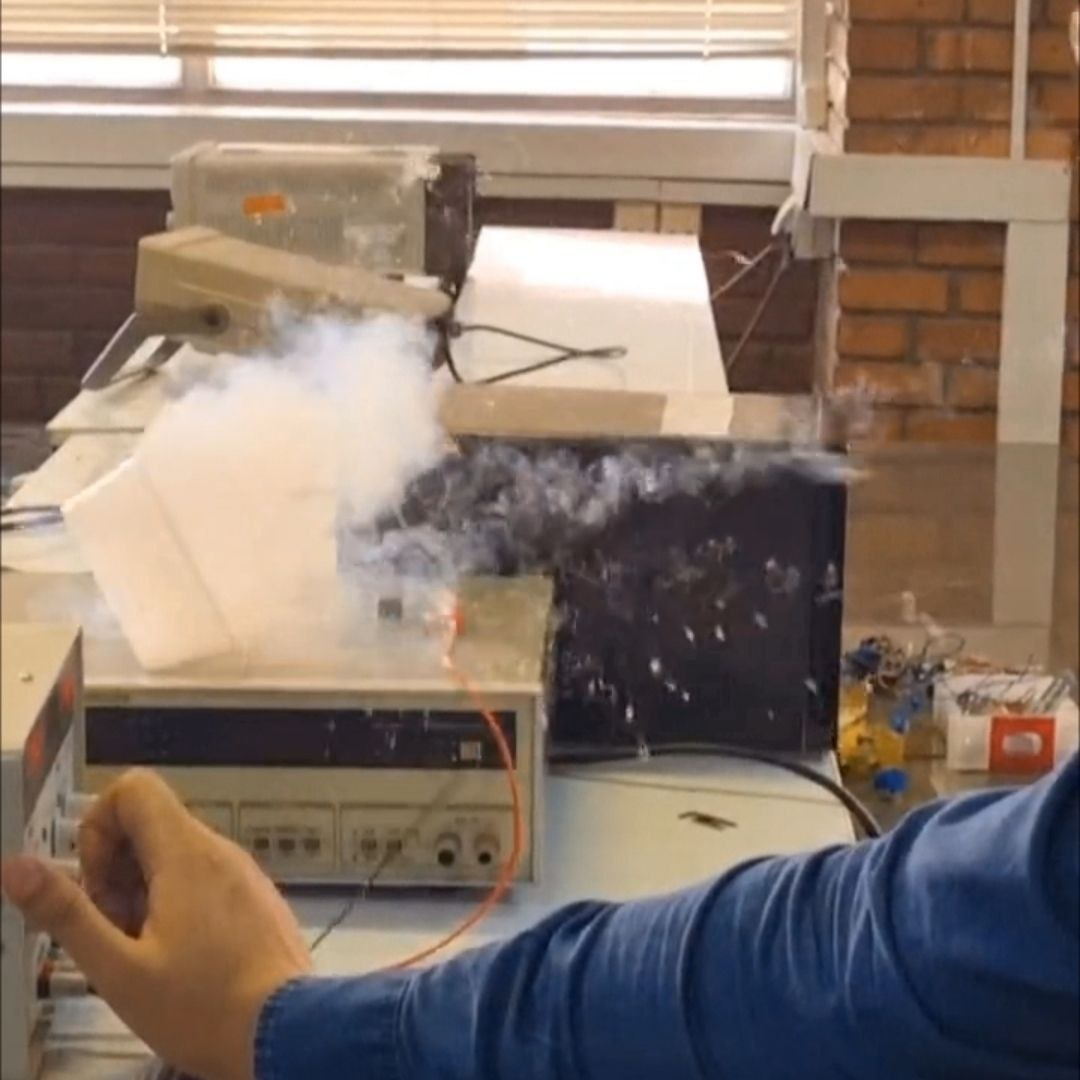
\includegraphics[scale=0.08,angle=0]{Fig/7.jpeg}
            \end{figure}
            
        }
    \end{subquestion}

    %--------------------------------------------
    \begin{subquestion}{Connect a $16$ V aluminum electrolytic capacitor inversely to a $16$ V DC voltage and observe the results.}
        \answer{}
    \end{subquestion}

\end{question}

%----------------------------------------------------------------------------------------
%	QUESTION 1
%----------------------------------------------------------------------------------------

\begin{question}

    \questiontext{Build the circuit shown in Fig. \ref{fig:cir2} on a breadboard, where $r=1$ k$\Omega$ denotes a resistor allowing to measure the current indirectly.}

    \begin{figure}[H]
        \centering
        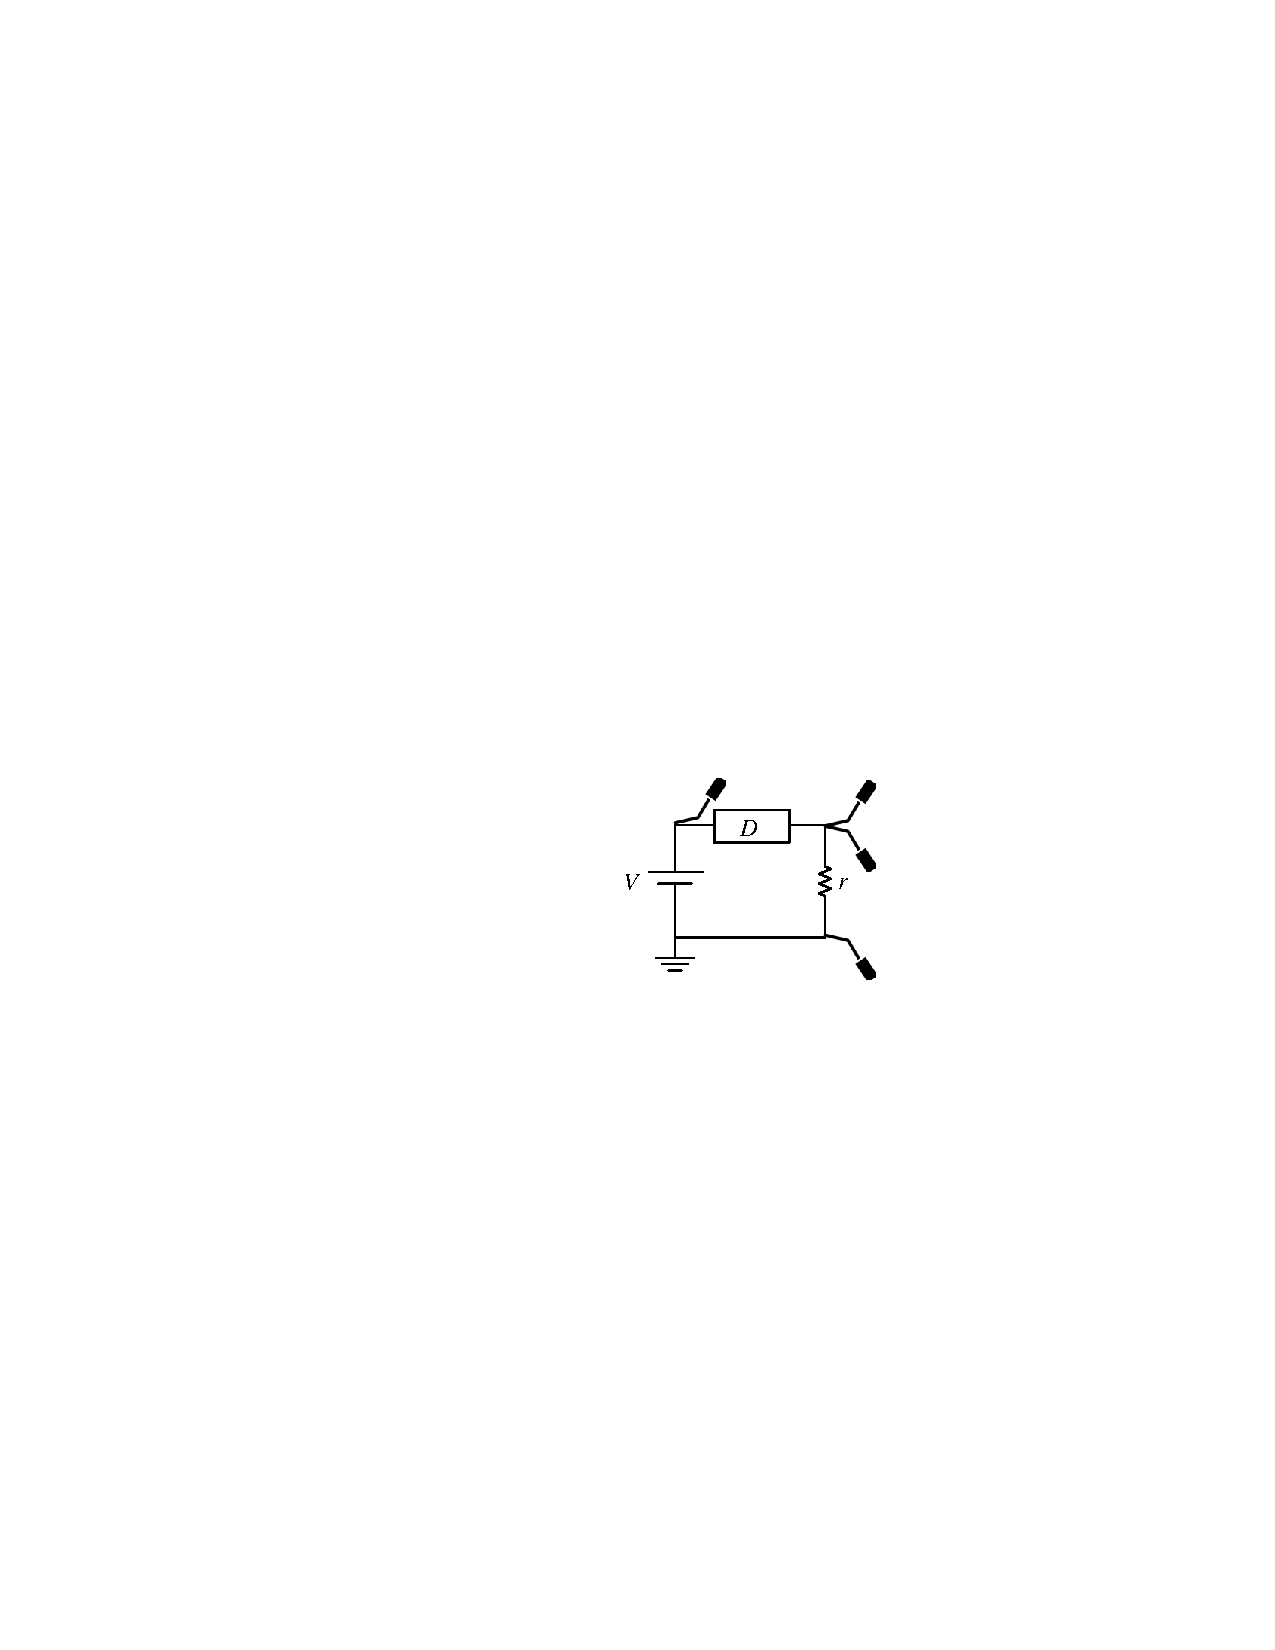
\includegraphics[scale=1.2,angle=0]{Fig/cir2.pdf}
        \caption{A test circuit for extracting the characteristic curve of a resistive element using multimeter.} \label{fig:cir2}
    \end{figure}

    %--------------------------------------------
    \begin{subquestion}{Replace $D$ with a $1$ k$\Omega$ resistor. Sweep the DC voltage over negative and positive ranges and record the voltage and current of the resistor using a multimeter. Use the recorded data to plot the characteristic curve of the resistor.}
        \answer{
            \begin{figure}[H]
                \centering
                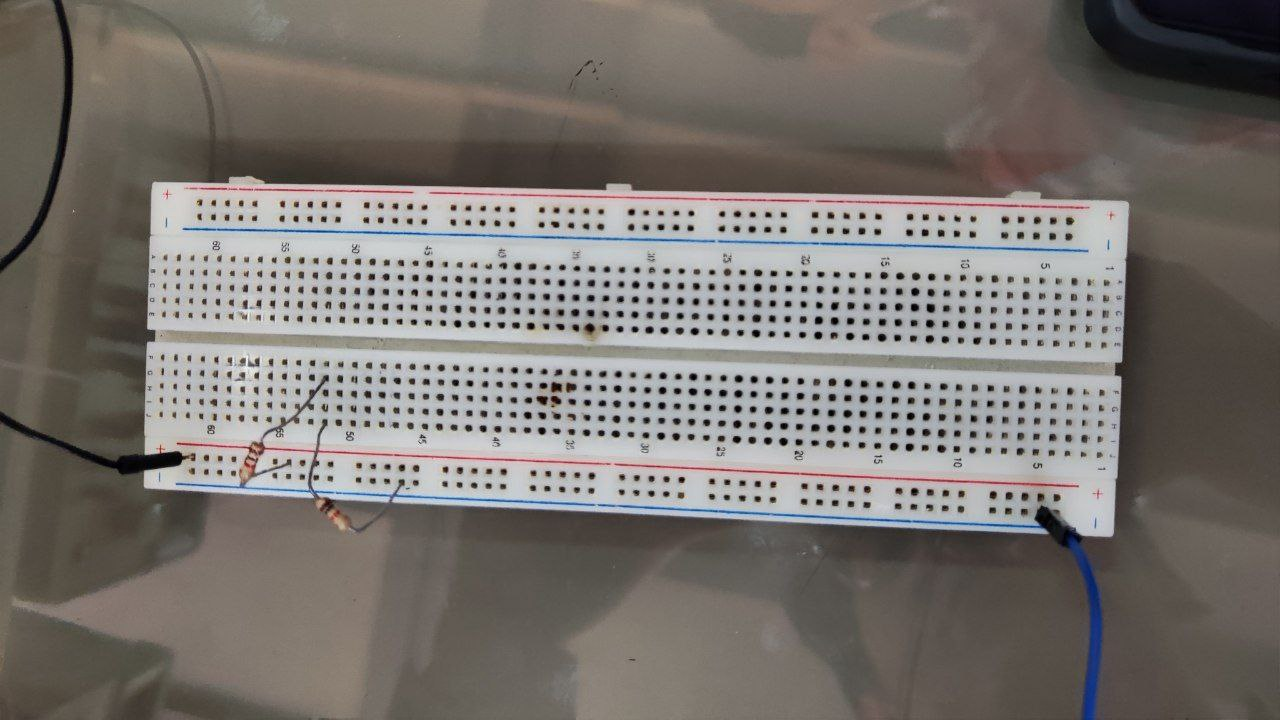
\includegraphics[scale=\PicScale,angle=0]{Fig/8.jpeg}
                \caption{The circuit.}
            \end{figure}

            \begin{figure}[H]
                \centering
                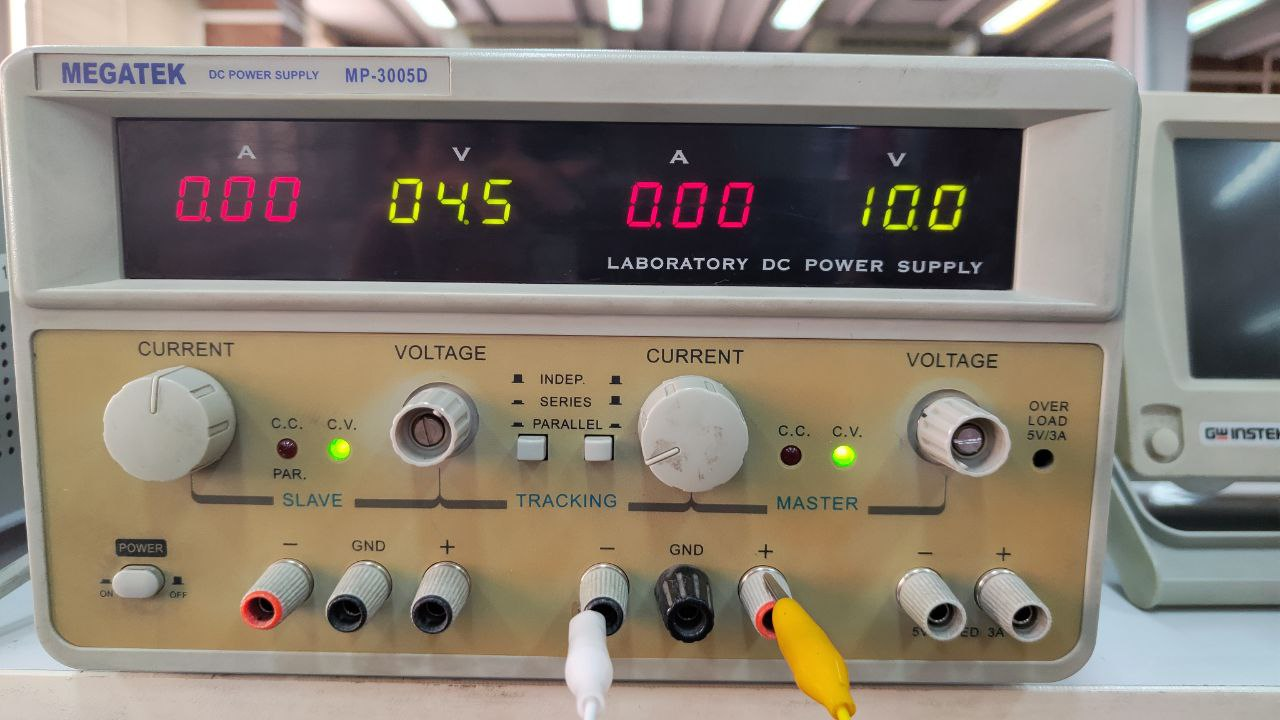
\includegraphics[scale=\PicScale,angle=0]{Fig/9.jpeg}
                \caption{DC power supply set to $10V$ and $-10V$.}
            \end{figure}
            \begin{figure}[H]
                \centering
                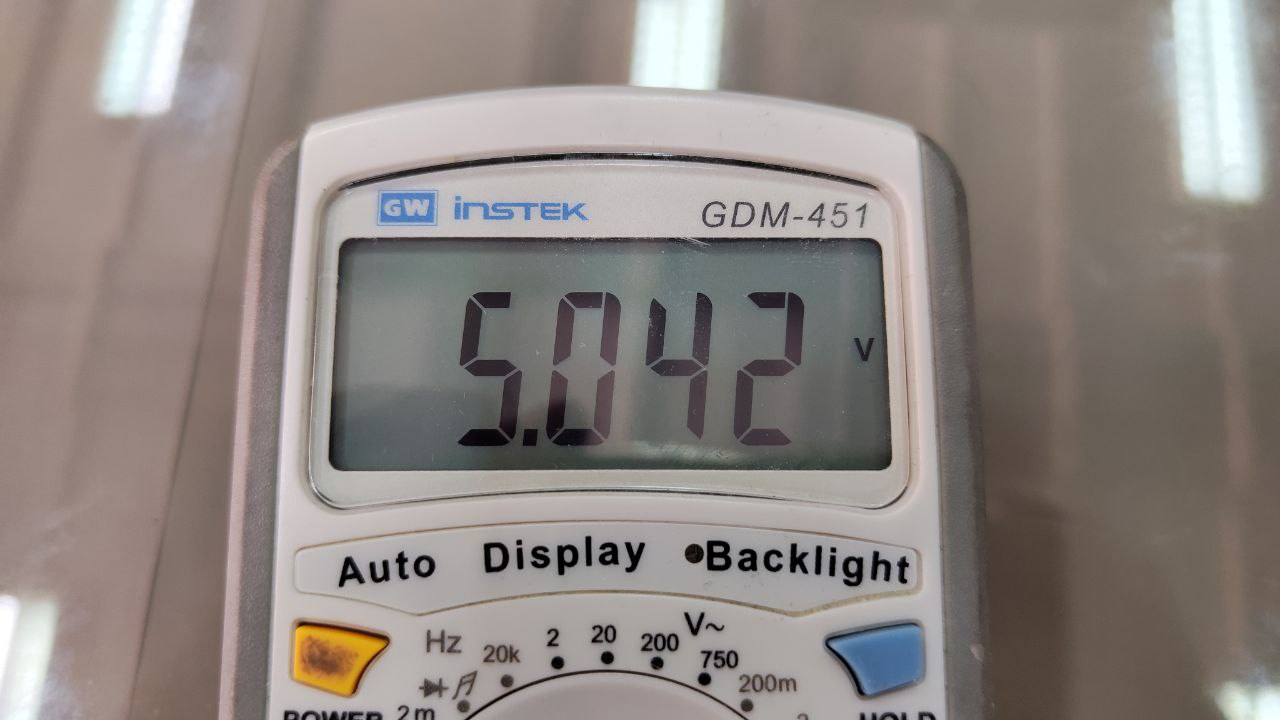
\includegraphics[scale=0.08,angle=0]{Fig/10.jpeg}
                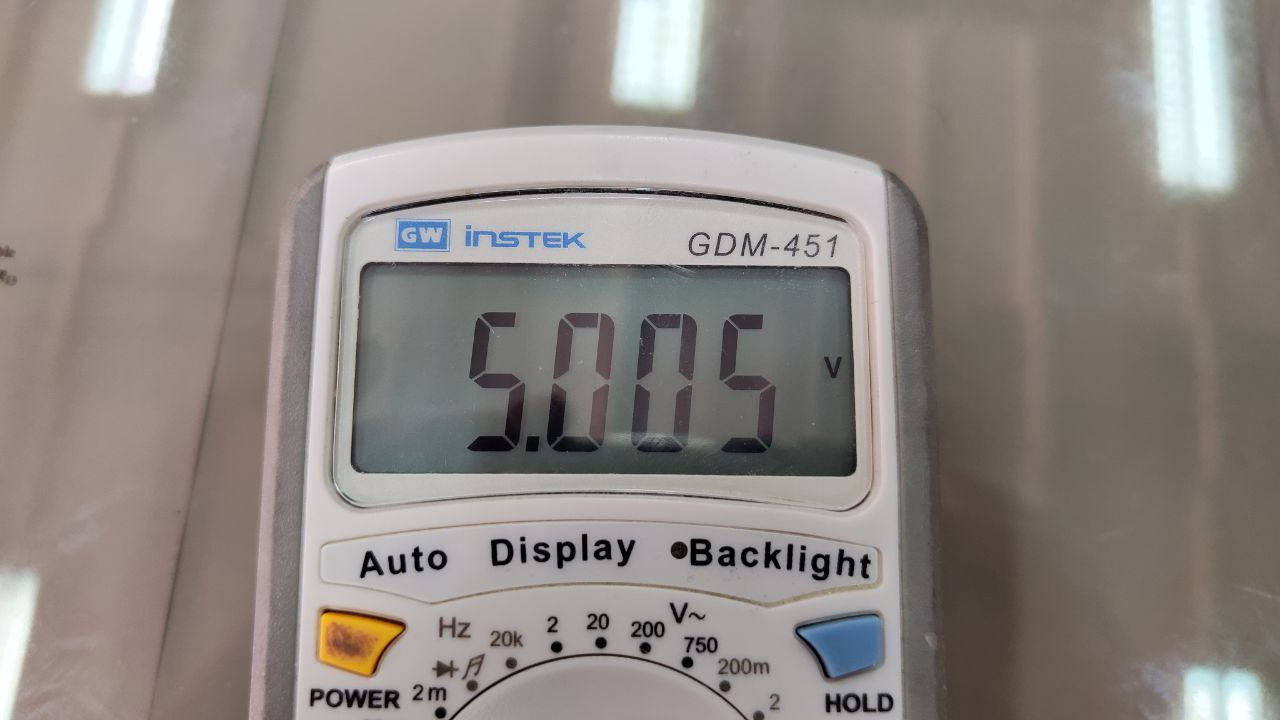
\includegraphics[scale=0.08,angle=0]{Fig/11.jpeg}
                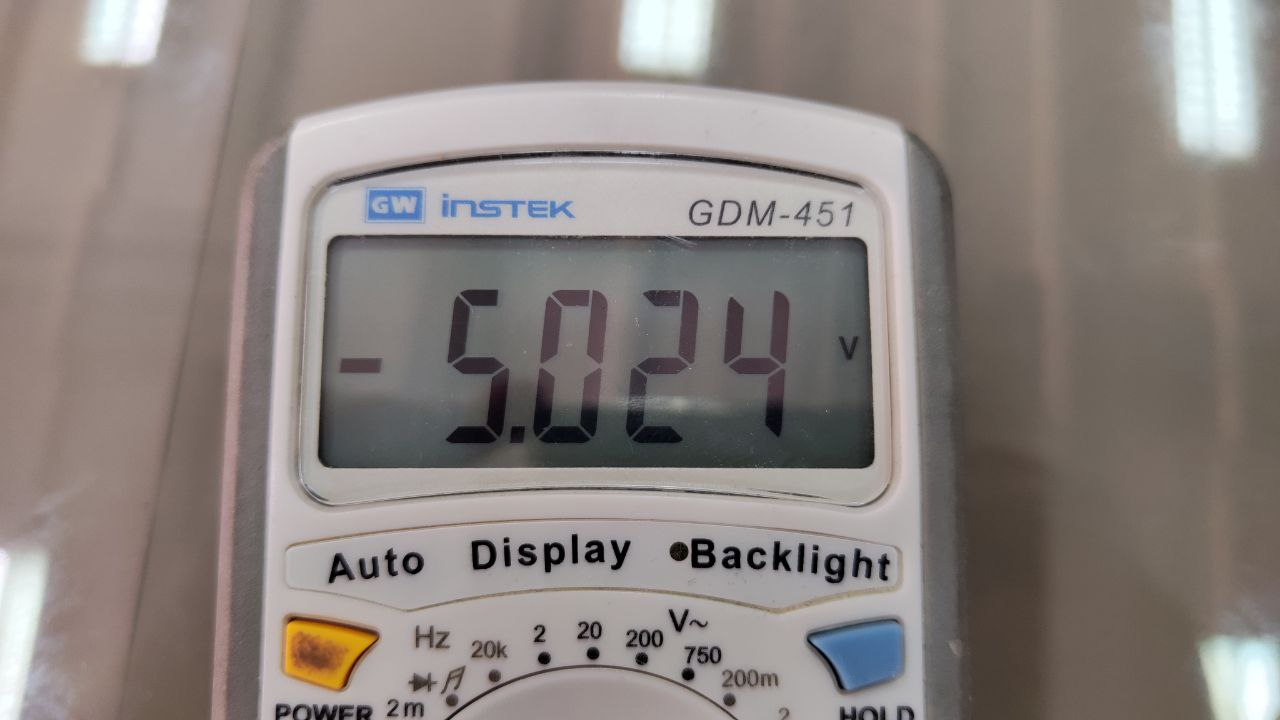
\includegraphics[scale=0.08,angle=0]{Fig/12.jpeg}
                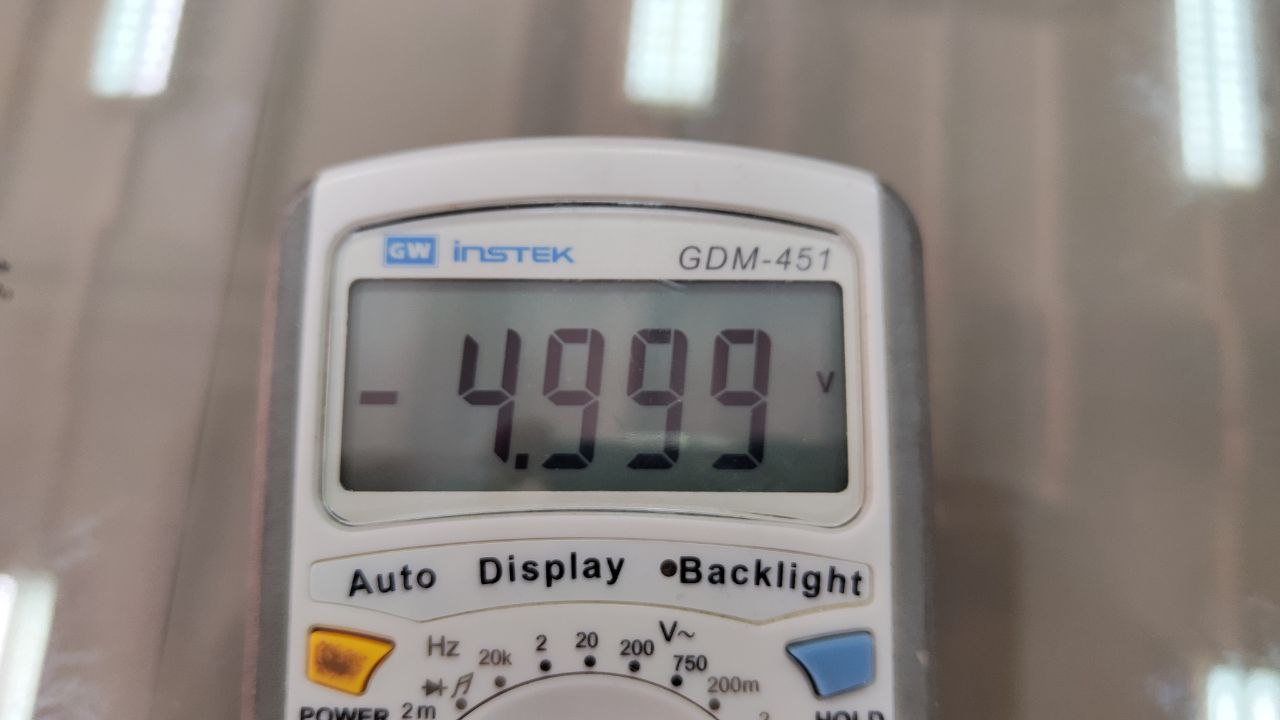
\includegraphics[scale=0.08,angle=0]{Fig/13.jpeg}
                \caption{First image is for D and $10V$, second image is for r and $10V$. \\
                \hspace*{14mm} Third image is for D and $-10V$, last image is for r and $-10V$.}
            \end{figure}
            \begin{figure}[H]
                \centering
                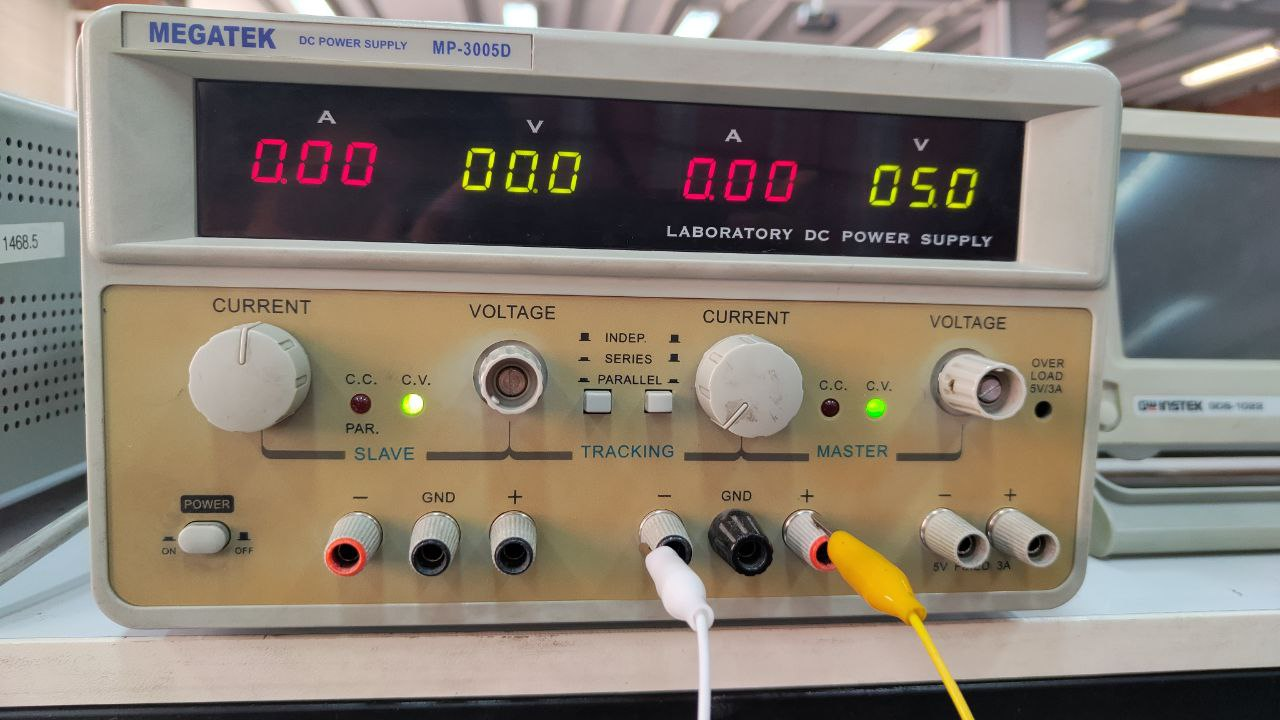
\includegraphics[scale=\PicScale,angle=0]{Fig/14.jpeg}
                \caption{DC power supply set to $5V$ and $-5V$.}
            \end{figure}
            \begin{figure}[H]
                \centering
                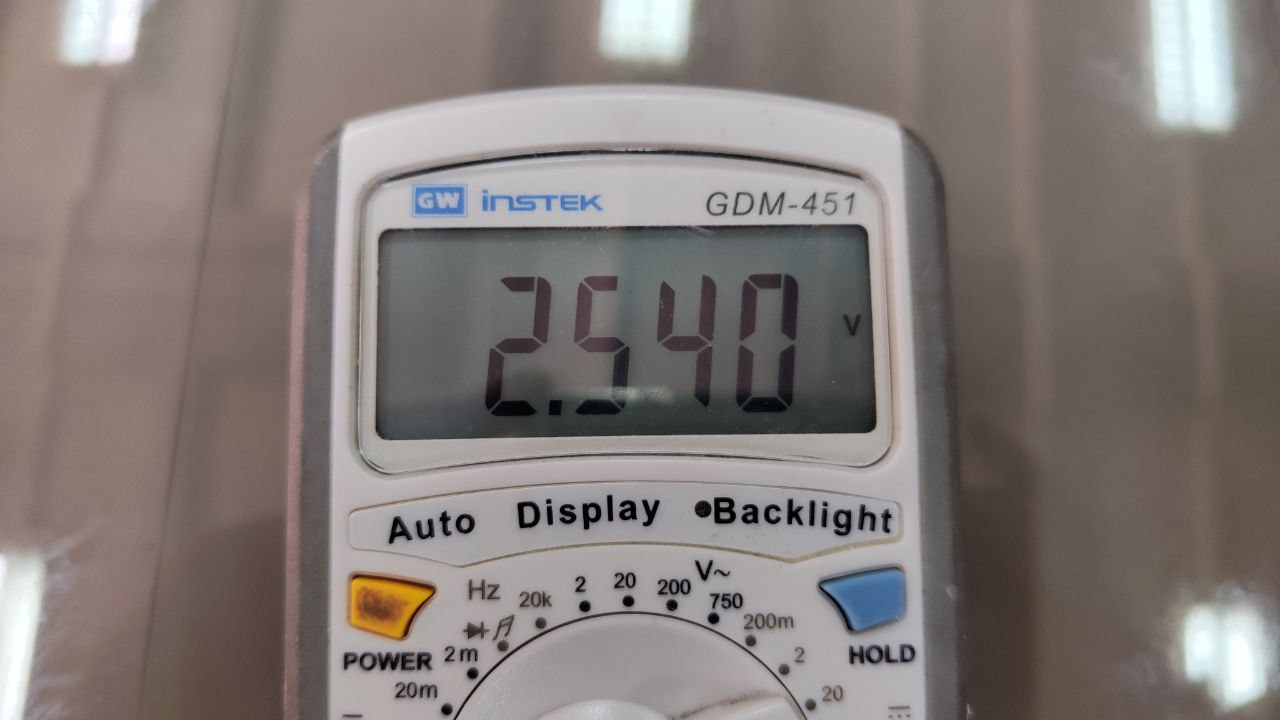
\includegraphics[scale=0.08,angle=0]{Fig/15.jpeg}
                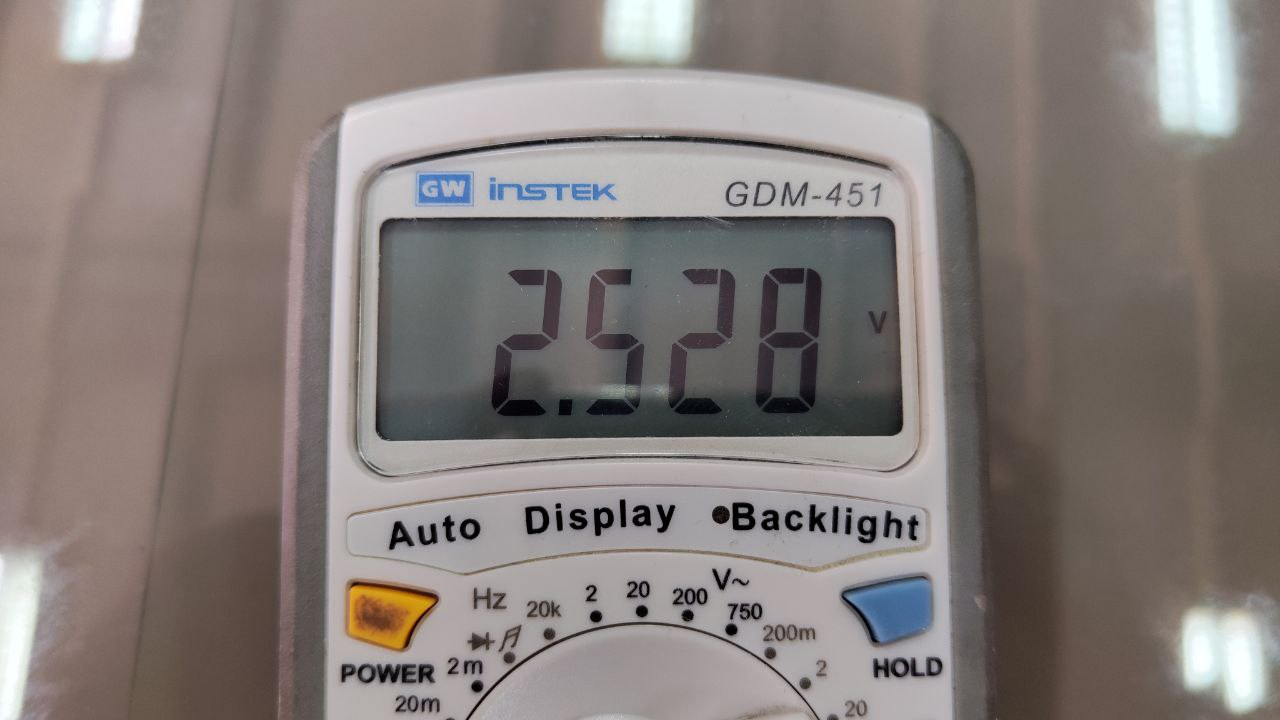
\includegraphics[scale=0.08,angle=0]{Fig/16.jpeg}
                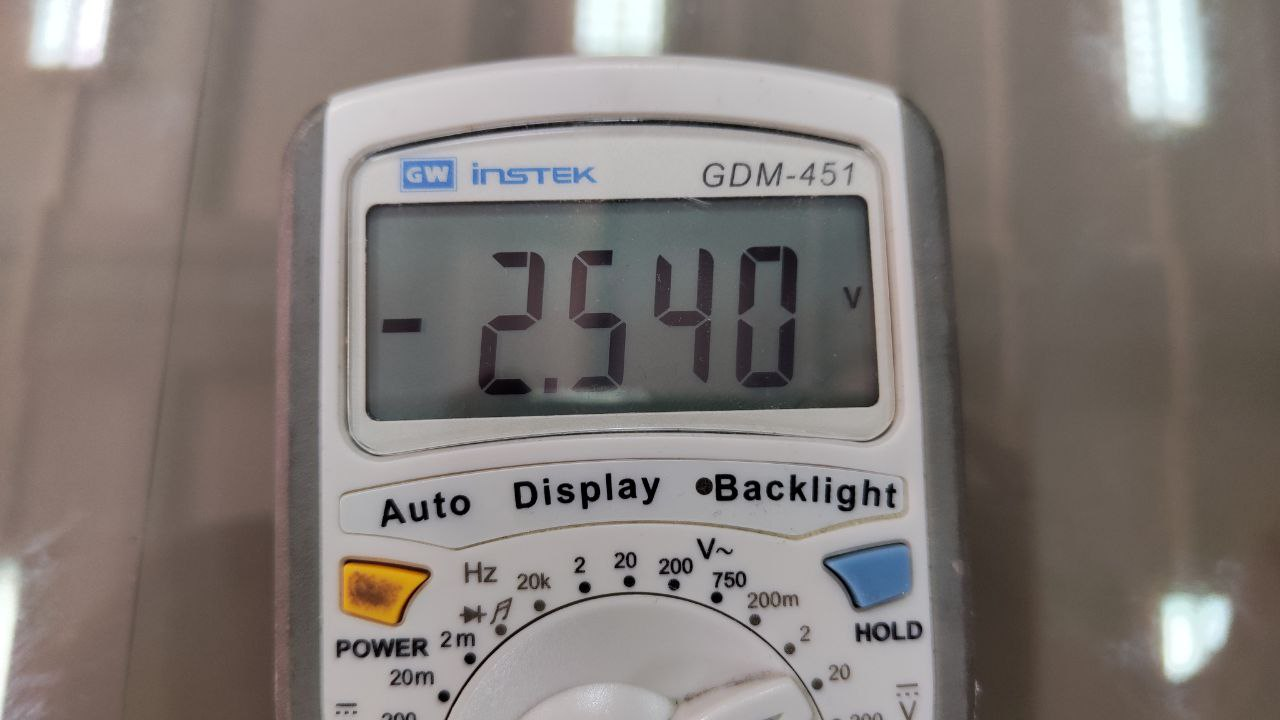
\includegraphics[scale=0.08,angle=0]{Fig/17.jpeg}
                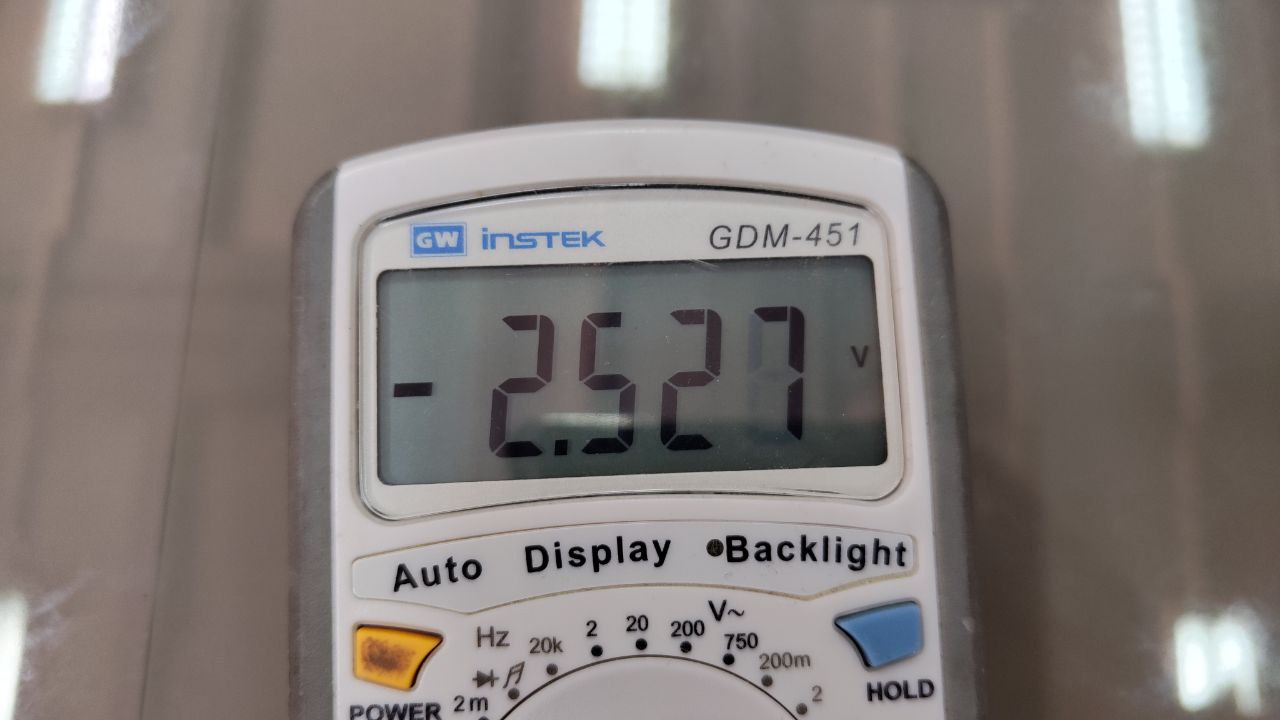
\includegraphics[scale=0.08,angle=0]{Fig/18.jpeg}
                \caption{First image is for D and $5V$, second image is for r and $5V$. \\
                \hspace*{14mm} Third image is for D and $-5V$, last image is for r and $-5V$.}
            \end{figure}
            \begin{figure}[H]
                \centering
                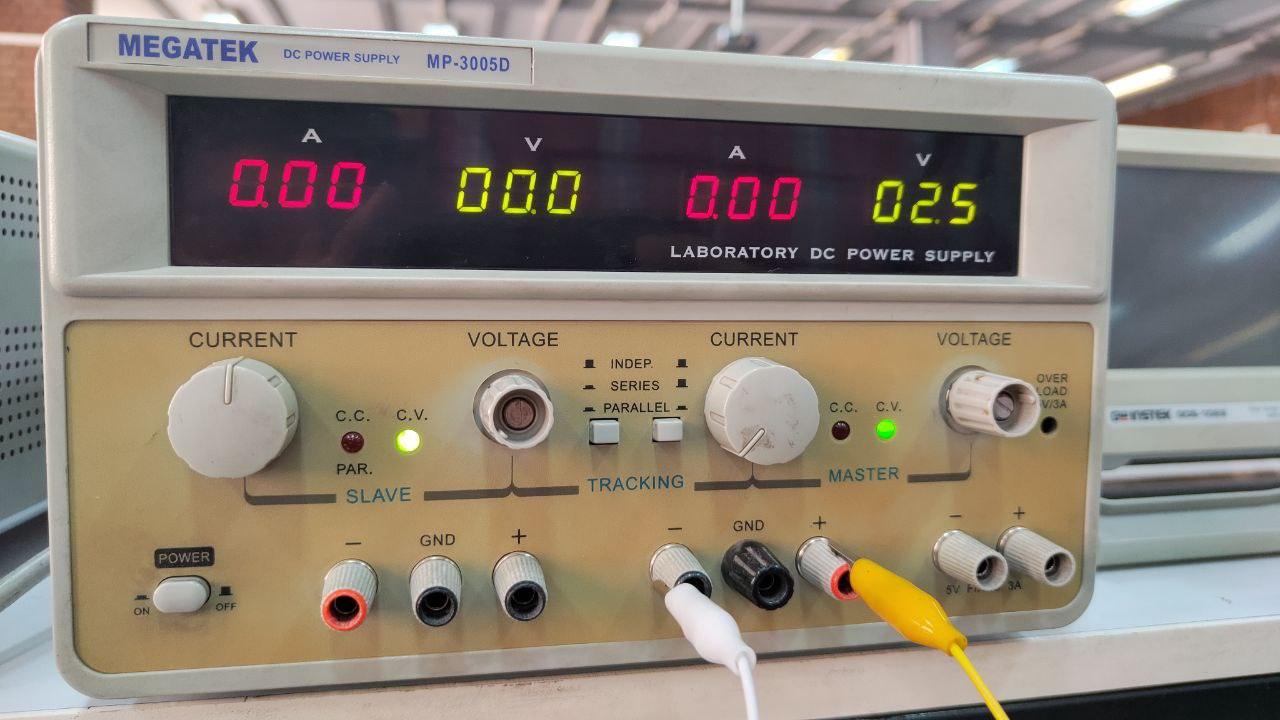
\includegraphics[scale=\PicScale,angle=0]{Fig/19.jpeg}
                \caption{DC power supply set to $2.5V$ and $-2.5V$.}
            \end{figure}
            \begin{figure}[H]
                \centering
                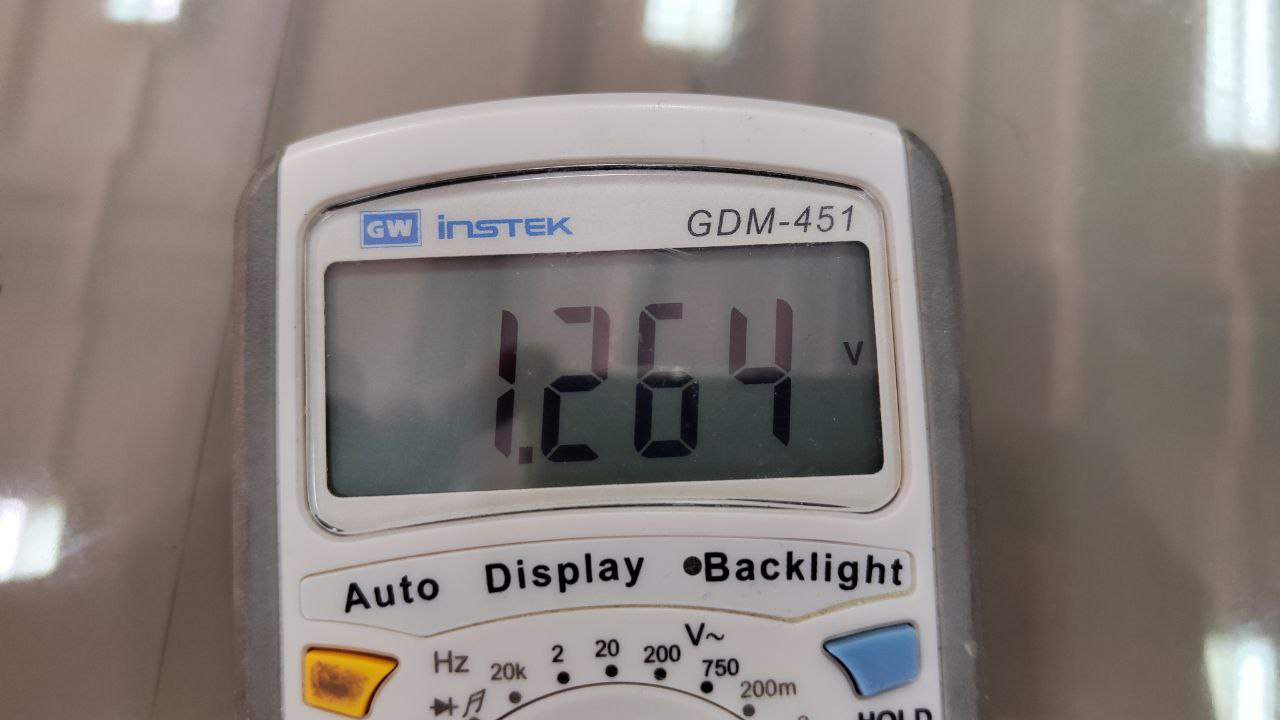
\includegraphics[scale=0.08,angle=0]{Fig/20.jpeg}
                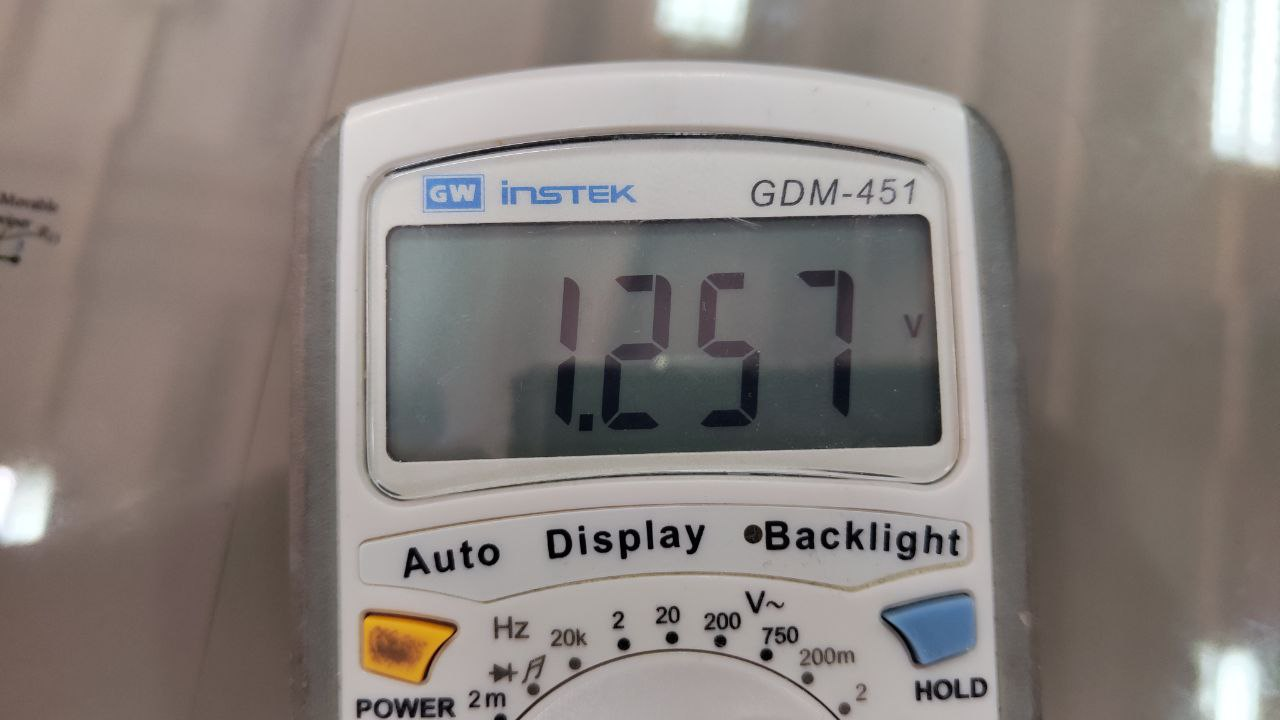
\includegraphics[scale=0.08,angle=0]{Fig/21.jpeg}
                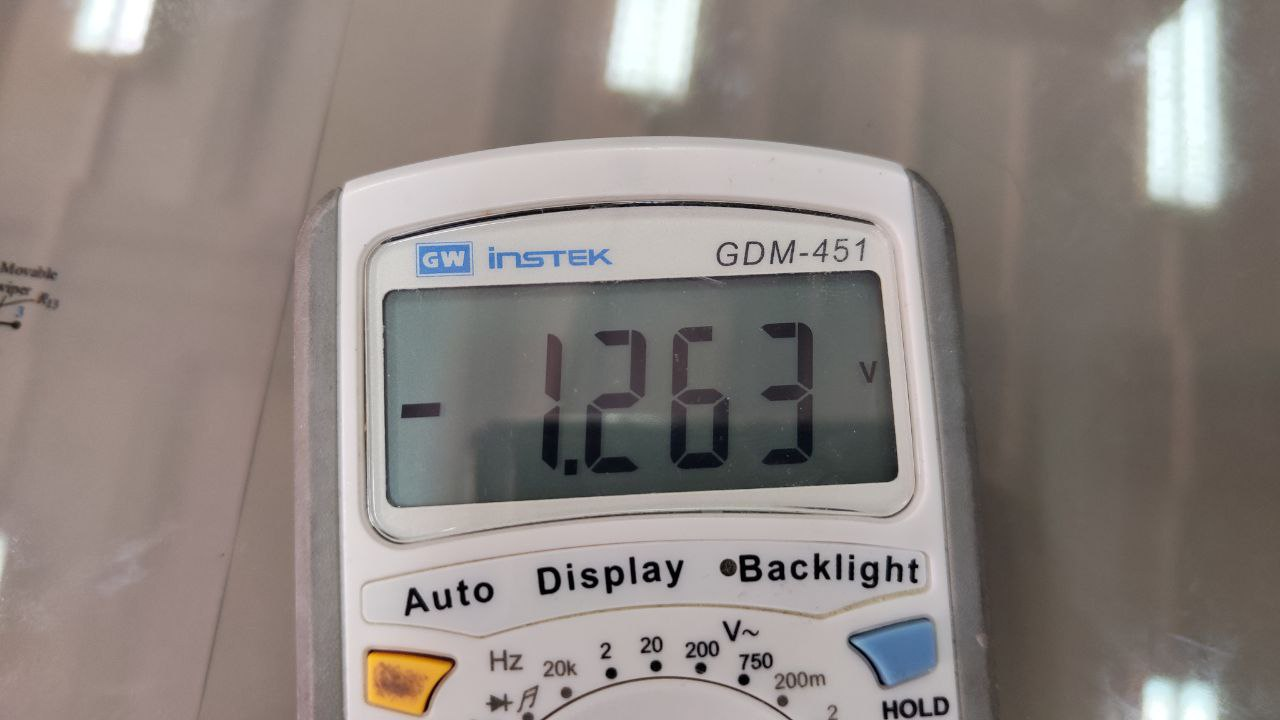
\includegraphics[scale=0.08,angle=0]{Fig/22.jpeg}
                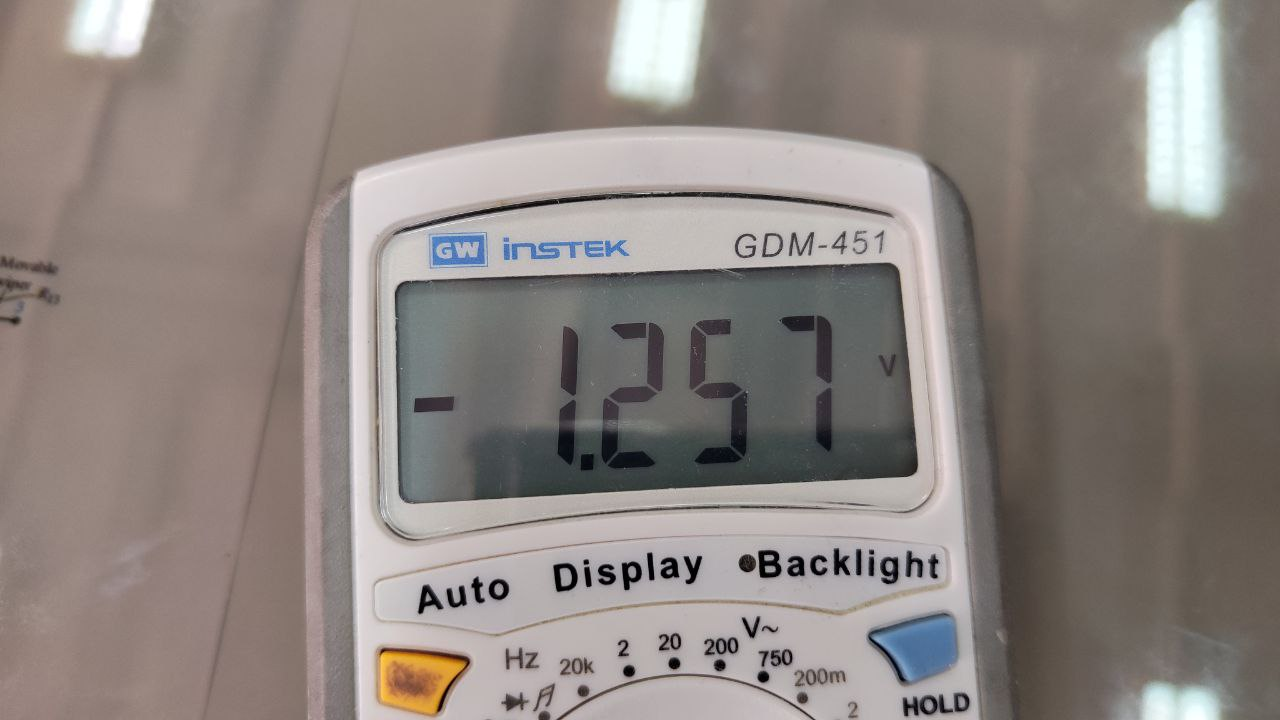
\includegraphics[scale=0.08,angle=0]{Fig/23.jpeg}
                \caption{First image is for D and $2.5V$, second image is for r and $2.5V$. \\
                \hspace*{14mm} Third image is for D and $-2.5V$, last image is for r and $-2.5V$.}
            \end{figure}

        }
    \end{subquestion}

    %--------------------------------------------
    \begin{subquestion}{Repeat the previous part for a diode.}
        \answer{
            \begin{figure}[H]
                \centering
                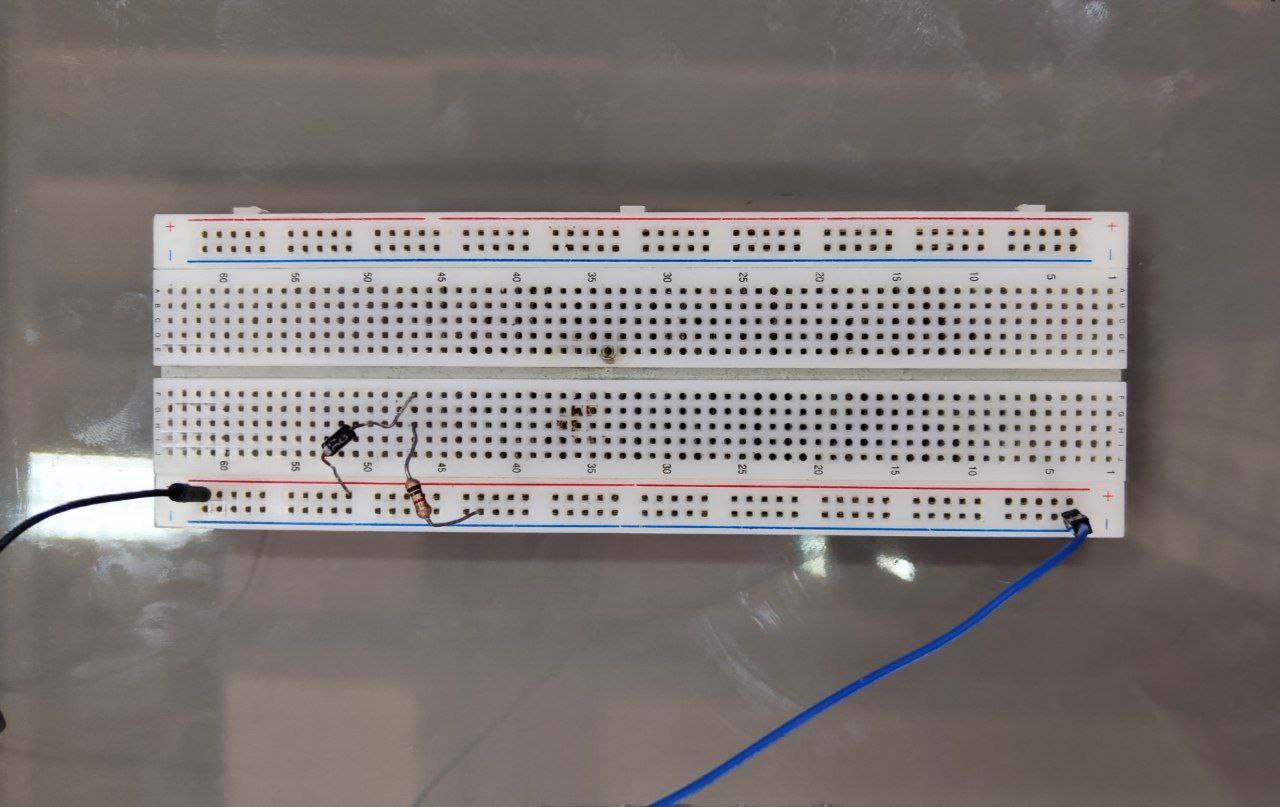
\includegraphics[scale=\PicScale,angle=0]{Fig/24.jpeg}
                \caption{The circuit.}
            \end{figure}

            \begin{figure}[H]
                \centering
                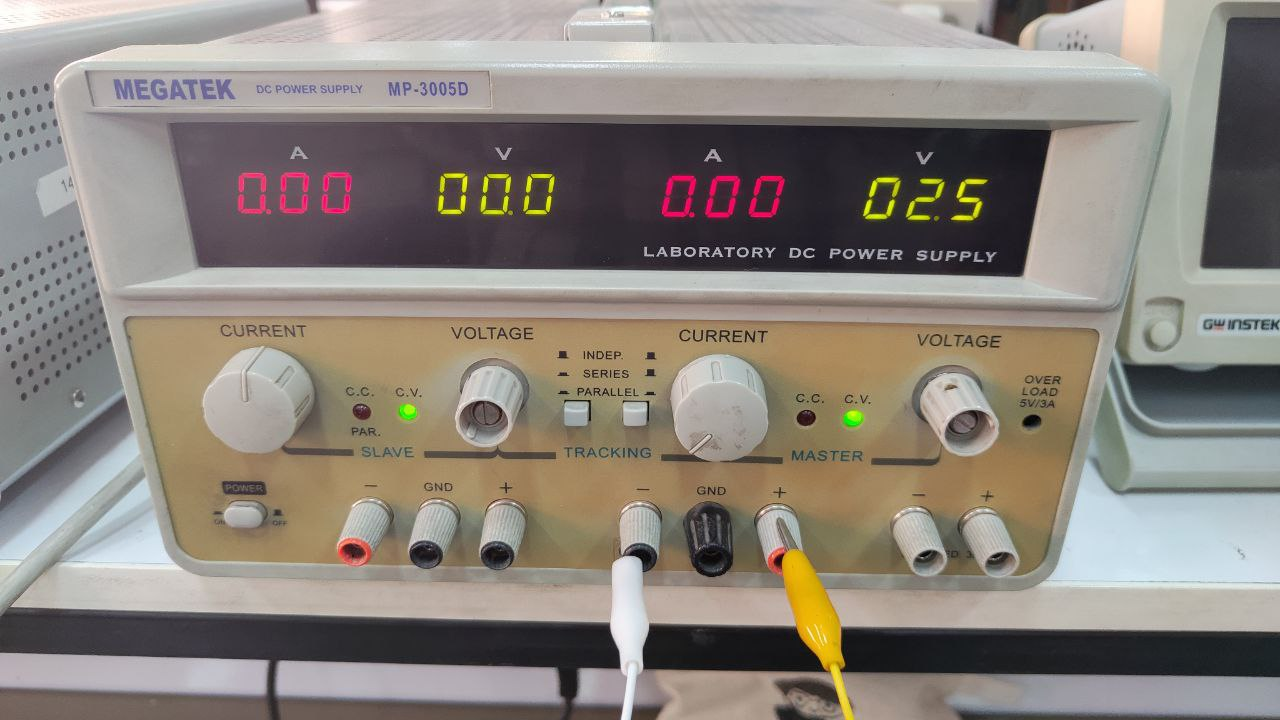
\includegraphics[scale=\PicScale,angle=0]{Fig/25.jpeg}
                \caption{DC power supply set to $10V$ and $-10V$.}
            \end{figure}
            \begin{figure}[H]
                \centering
                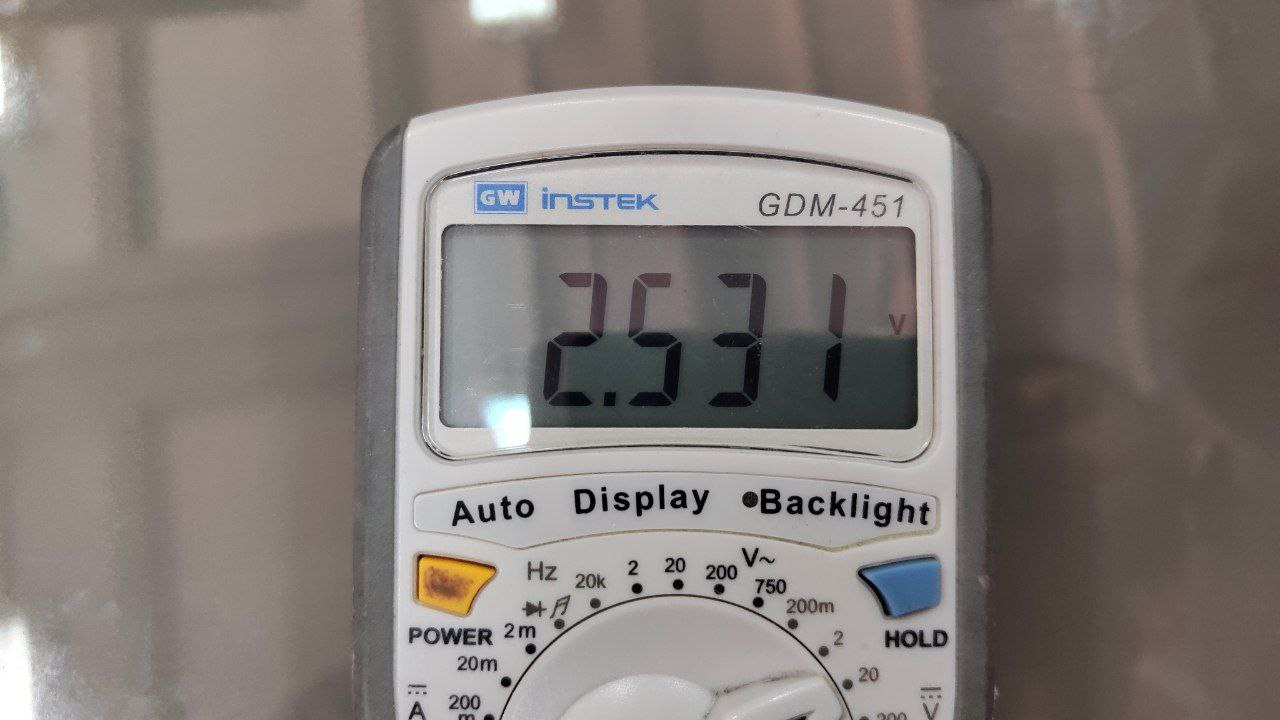
\includegraphics[scale=0.08,angle=0]{Fig/26.jpeg}
                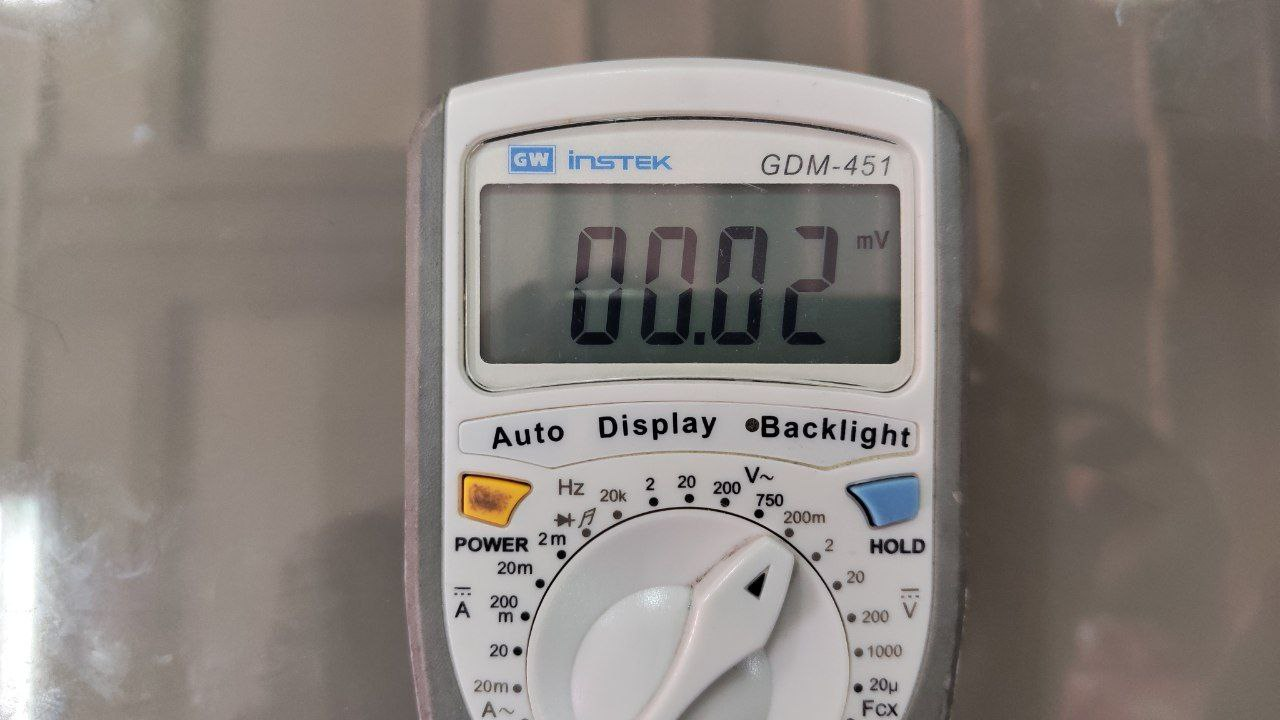
\includegraphics[scale=0.08,angle=0]{Fig/27.jpeg}
                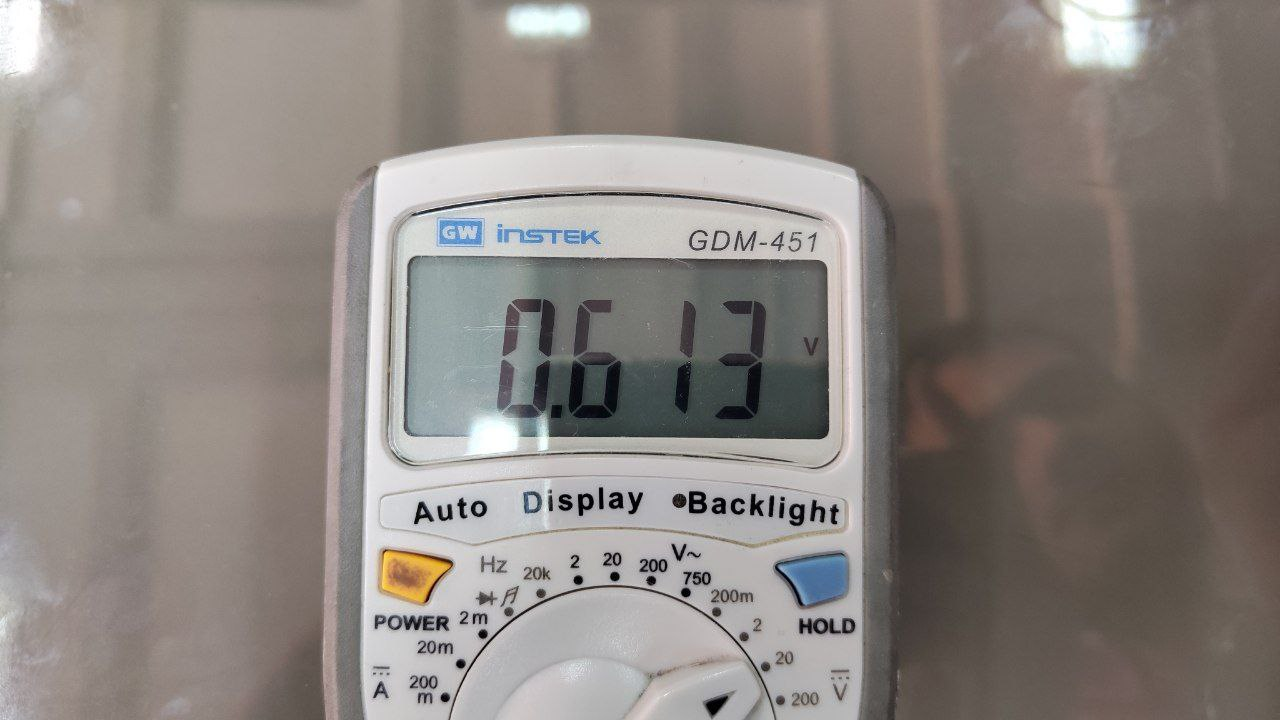
\includegraphics[scale=0.08,angle=0]{Fig/28.jpeg}
                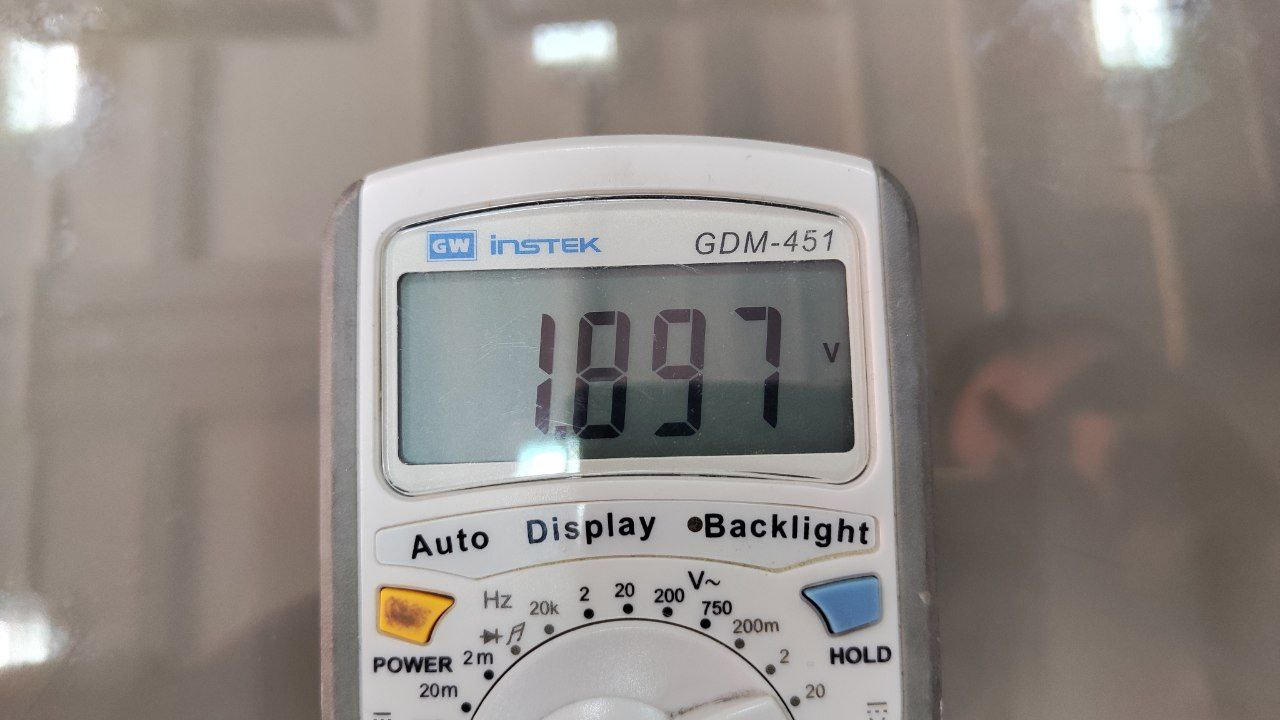
\includegraphics[scale=0.08,angle=0]{Fig/29.jpeg}
                \caption{First image is for D and $10V$, second image is for r and $10V$. \\
                \hspace*{14mm} Third image is for D and $-10V$, last image is for r and $-10V$.}
            \end{figure}
            \begin{figure}[H]
                \centering
                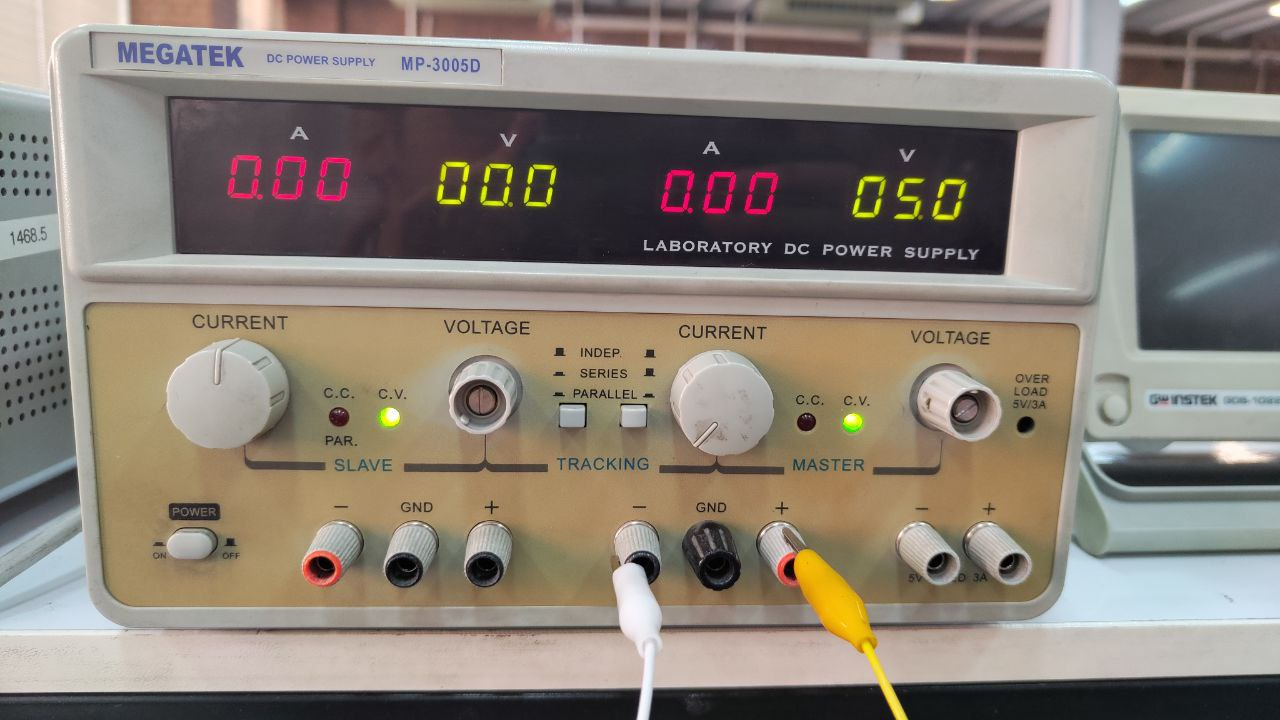
\includegraphics[scale=\PicScale,angle=0]{Fig/30.jpeg}
                \caption{DC power supply set to $5V$ and $-5V$.}
            \end{figure}
            \begin{figure}[H]
                \centering
                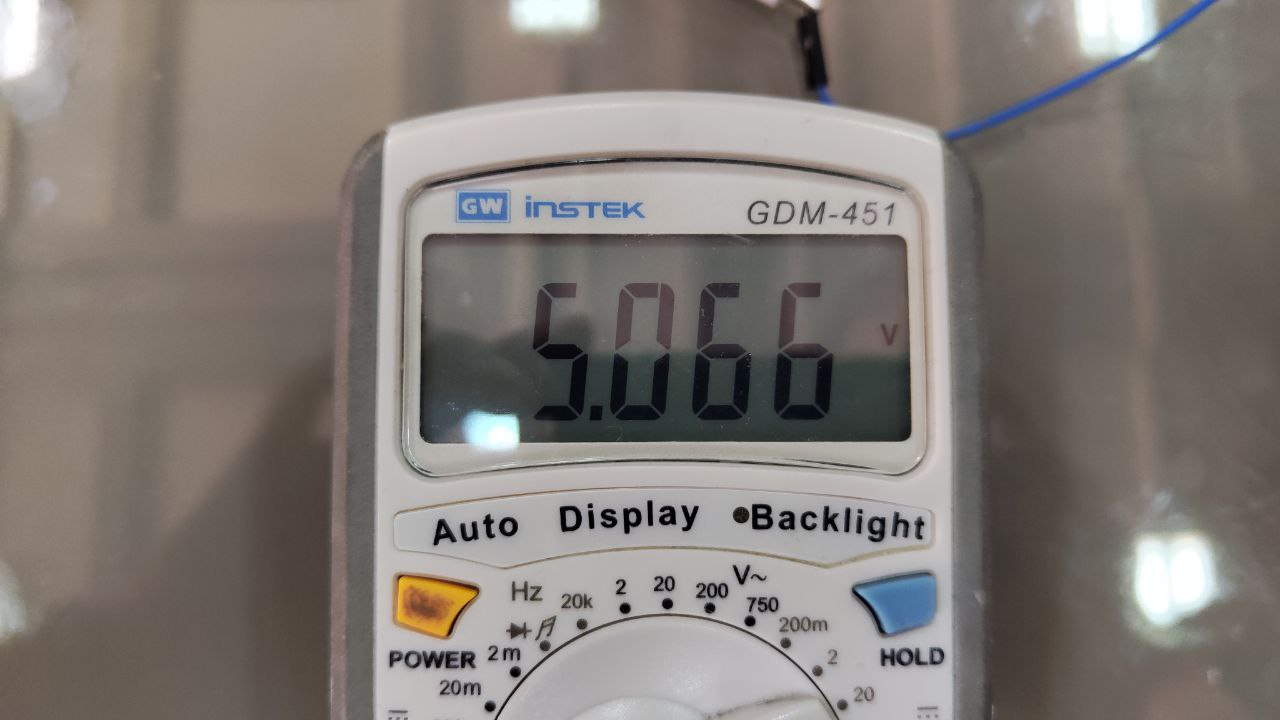
\includegraphics[scale=0.08,angle=0]{Fig/31.jpeg}
                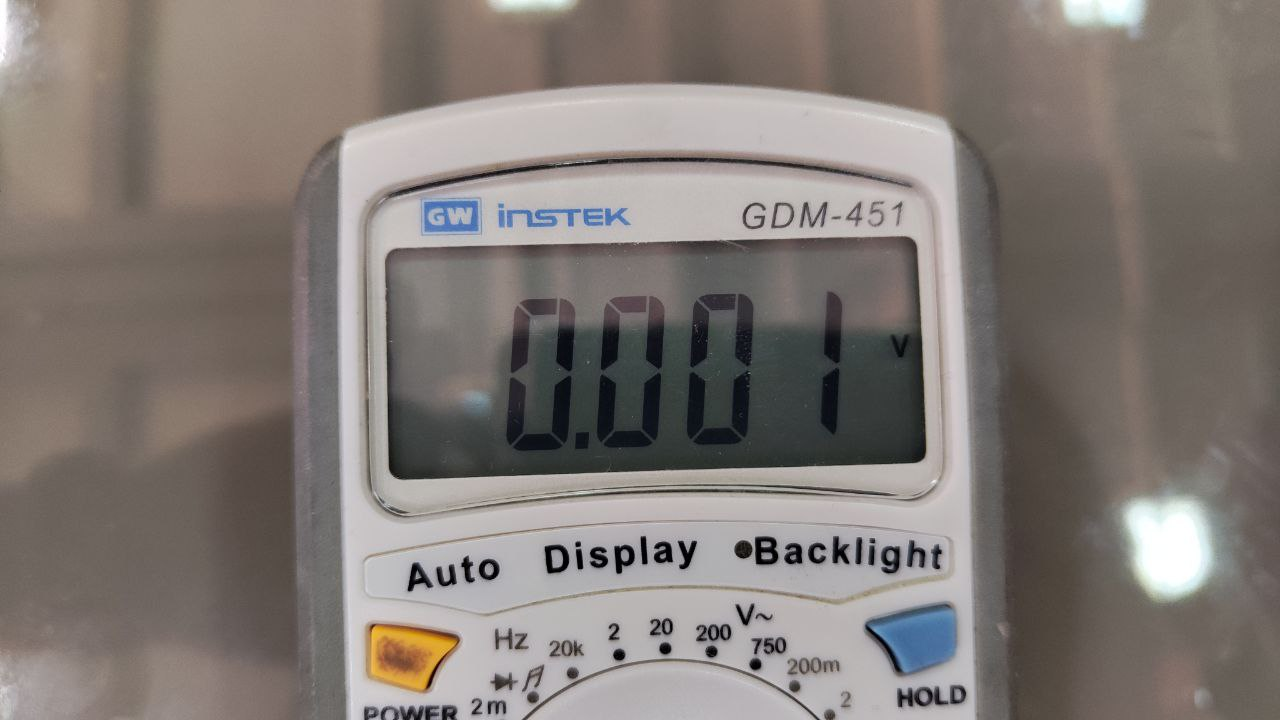
\includegraphics[scale=0.08,angle=0]{Fig/32.jpeg}
                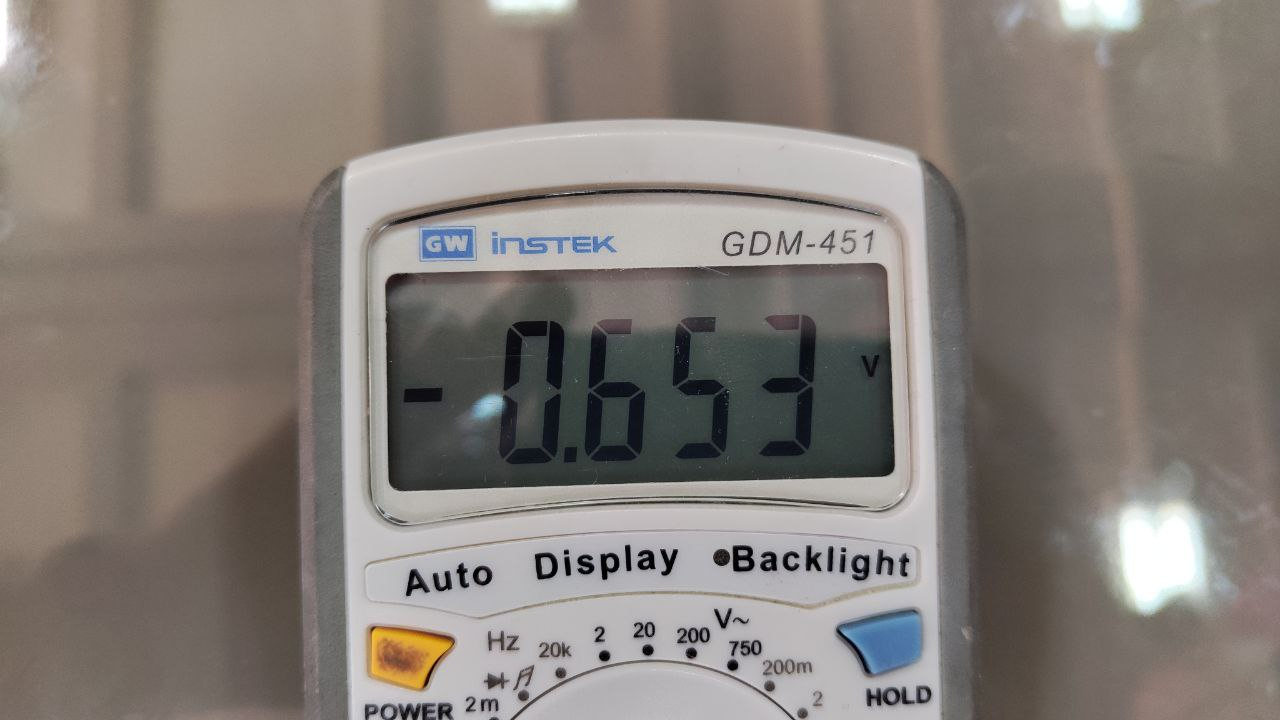
\includegraphics[scale=0.08,angle=0]{Fig/33.jpeg}
                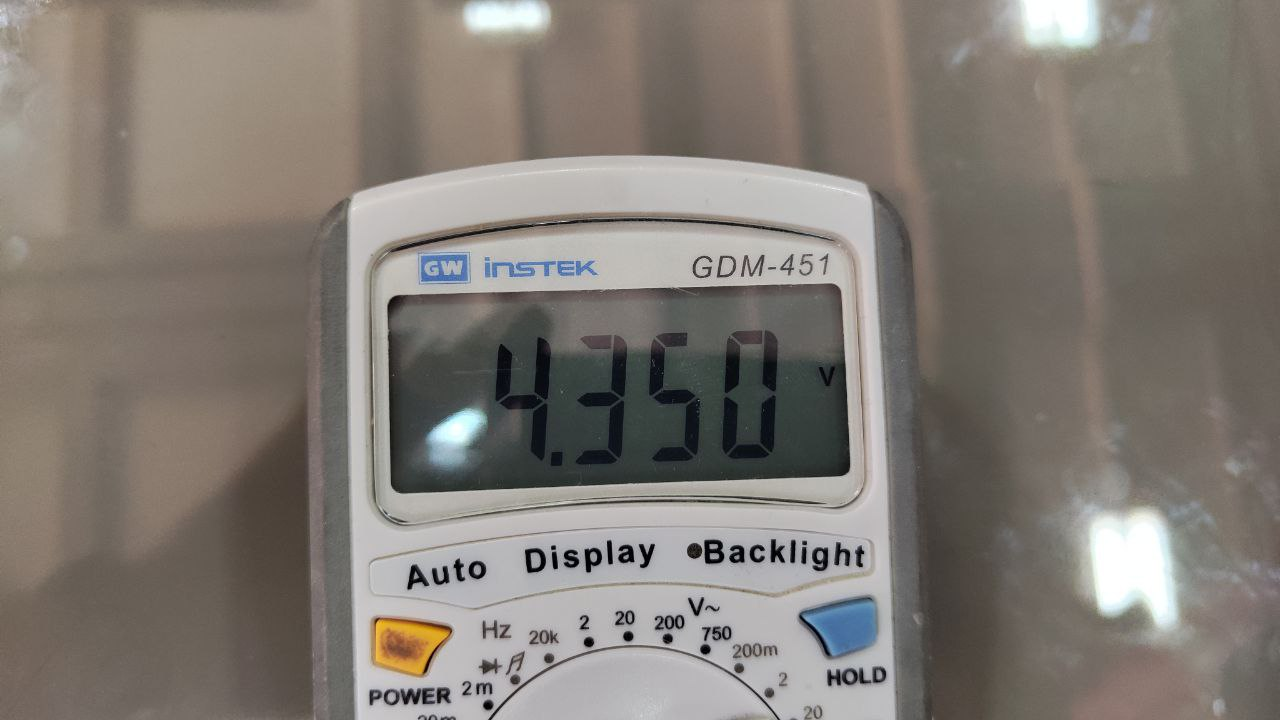
\includegraphics[scale=0.08,angle=0]{Fig/34.jpeg}
                \caption{First image is for D and $5V$, second image is for r and $5V$. \\
                \hspace*{14mm} Third image is for D and $-5V$, last image is for r and $-5V$.}
            \end{figure}
            \begin{figure}[H]
                \centering
                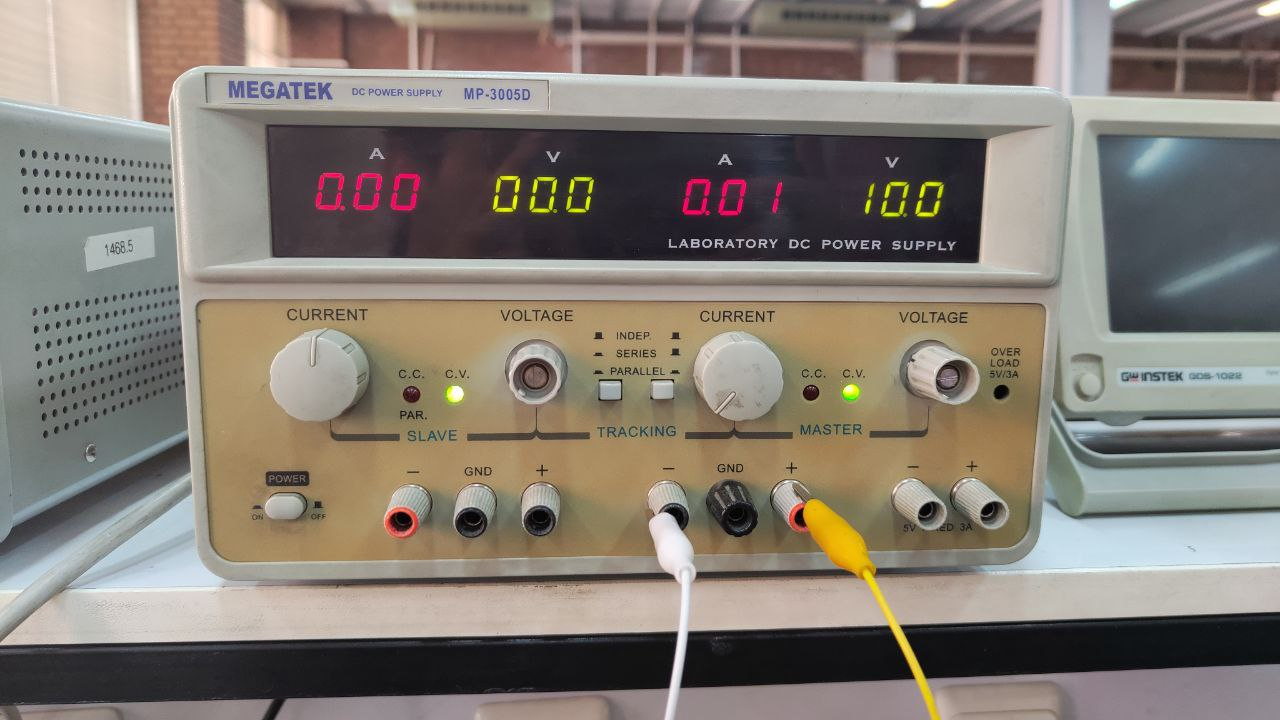
\includegraphics[scale=\PicScale,angle=0]{Fig/35.jpeg}
                \caption{DC power supply set to $2.5V$ and $-2.5V$.}
            \end{figure}
            \begin{figure}[H]
                \centering
                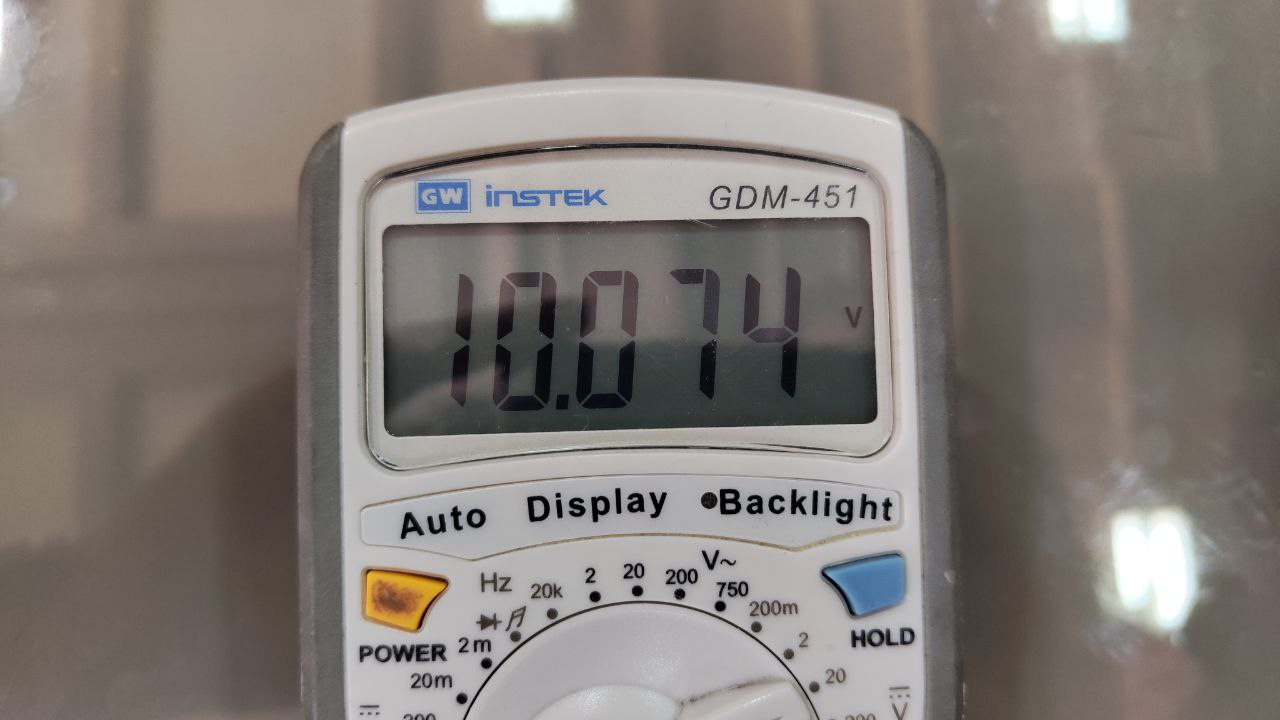
\includegraphics[scale=0.08,angle=0]{Fig/36.jpeg}
                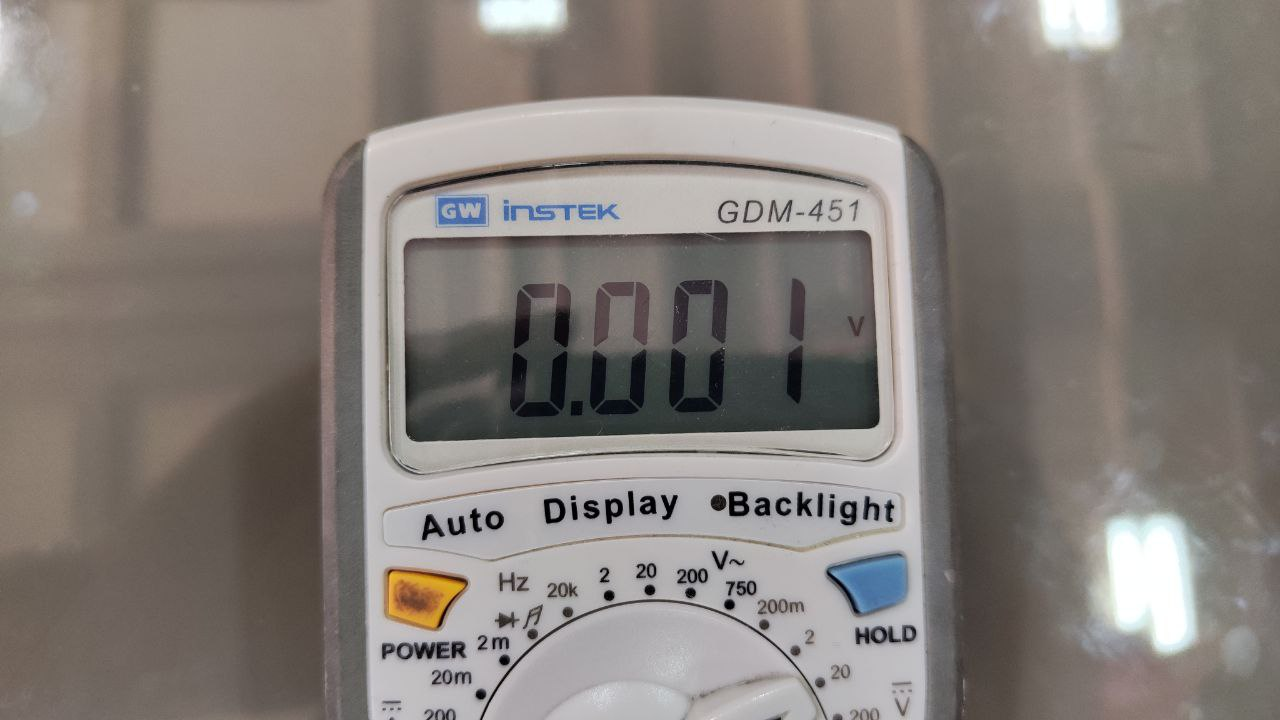
\includegraphics[scale=0.08,angle=0]{Fig/37.jpeg}
                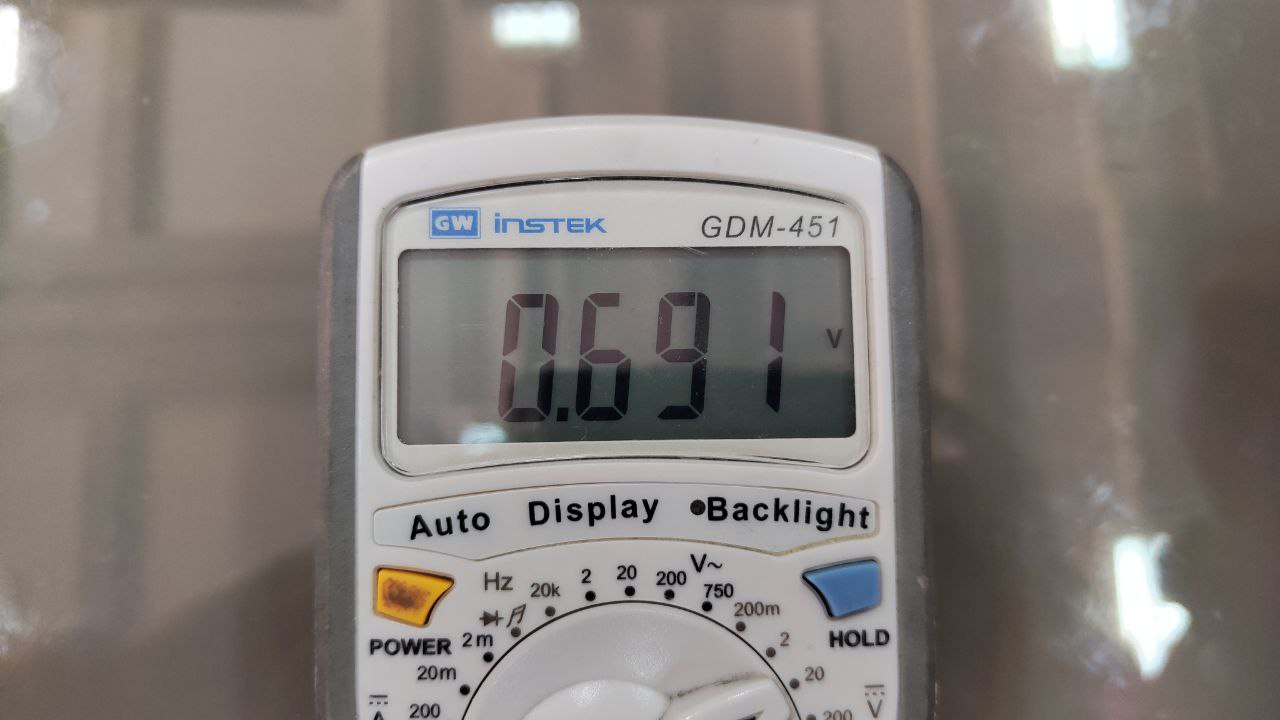
\includegraphics[scale=0.08,angle=0]{Fig/38.jpeg}
                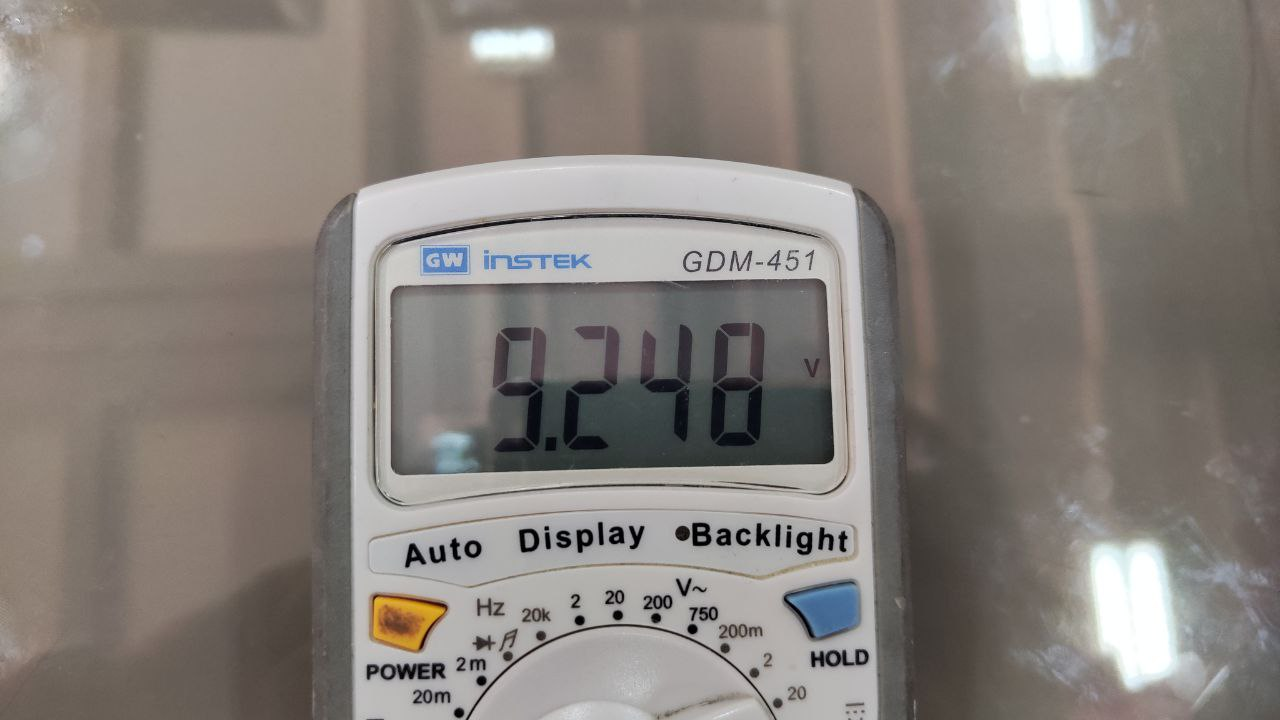
\includegraphics[scale=0.08,angle=0]{Fig/39.jpeg}
                \caption{First image is for D and $2.5V$, second image is for r and $2.5V$. \\
                \hspace*{14mm} Third image is for D and $-2.5V$, last image is for r and $-2.5V$.}
            \end{figure}

        }
    \end{subquestion}


\end{question}


%----------------------------------------------------------------------------------------
%	QUESTION 1
%----------------------------------------------------------------------------------------

\begin{question}

    \questiontext{The experimental setup of Fig. \ref{fig:cir3} is used to display the Lissajous curve constructed by $v_x(t)$ and
        $v_y(t)$, where $D$ is a basic circuit element and $r=1$ k$\Omega$. }

    \begin{figure}[H]
        \centering
        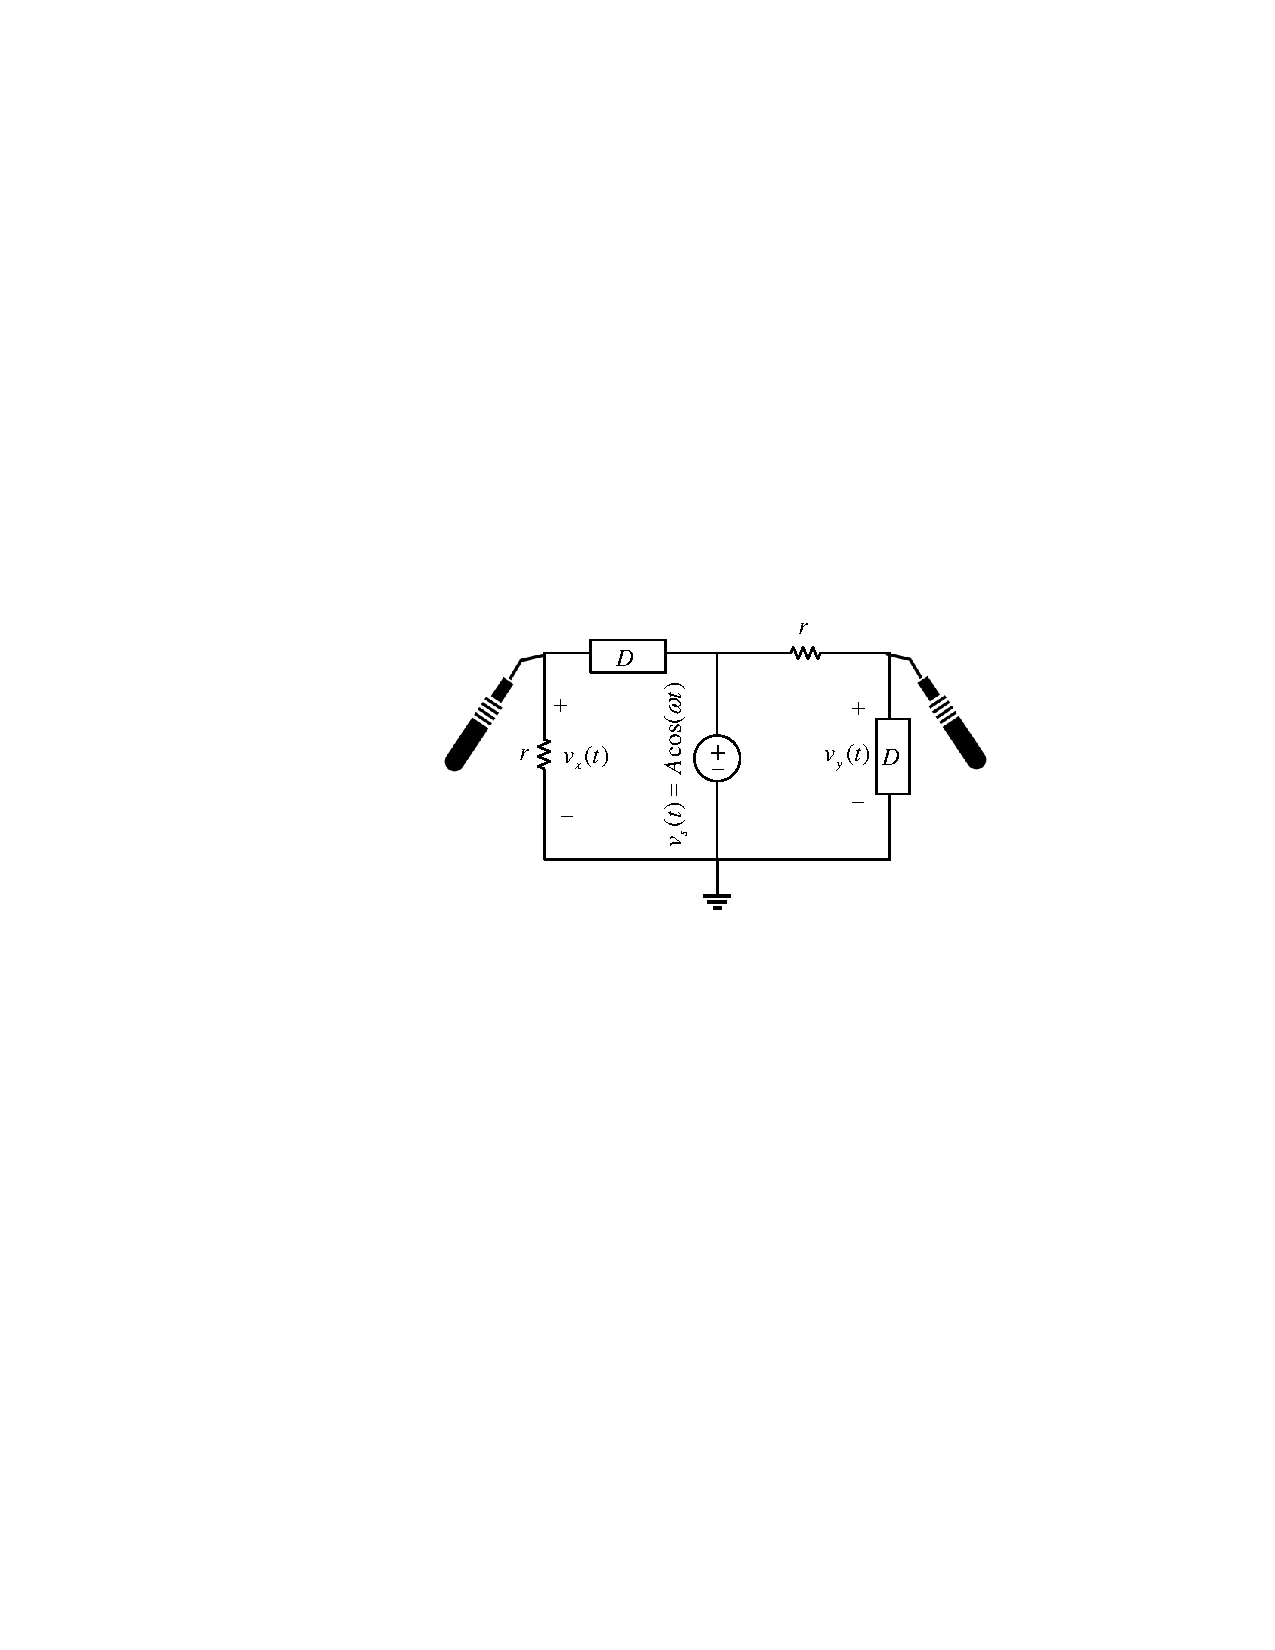
\includegraphics[scale=1.2,angle=0]{Fig/cir3.pdf}
        \caption{A test circuit for extracting the characteristic curve of a resistive element using oscilloscope.} \label{fig:cir3}
    \end{figure}

    %--------------------------------------------
    \begin{subquestion}{How can the displayed Lissajous curve be used
            to obtain the characteristic curve of a resistive element?}
        \answer{}
    \end{subquestion}

    %--------------------------------------------
    \begin{subquestion}{Can the characteristic curve be extracted using the circuit of Fig. \ref{fig:cir2} and an oscilloscope? }
        \answer{}
    \end{subquestion}

    %--------------------------------------------
    \begin{subquestion}{Replace $D$ with a $1$ k$\Omega$ resistor and see the corresponding characteristic curve on the oscilloscope screen.}
        \answer{
            \begin{figure}[H]
                \centering
                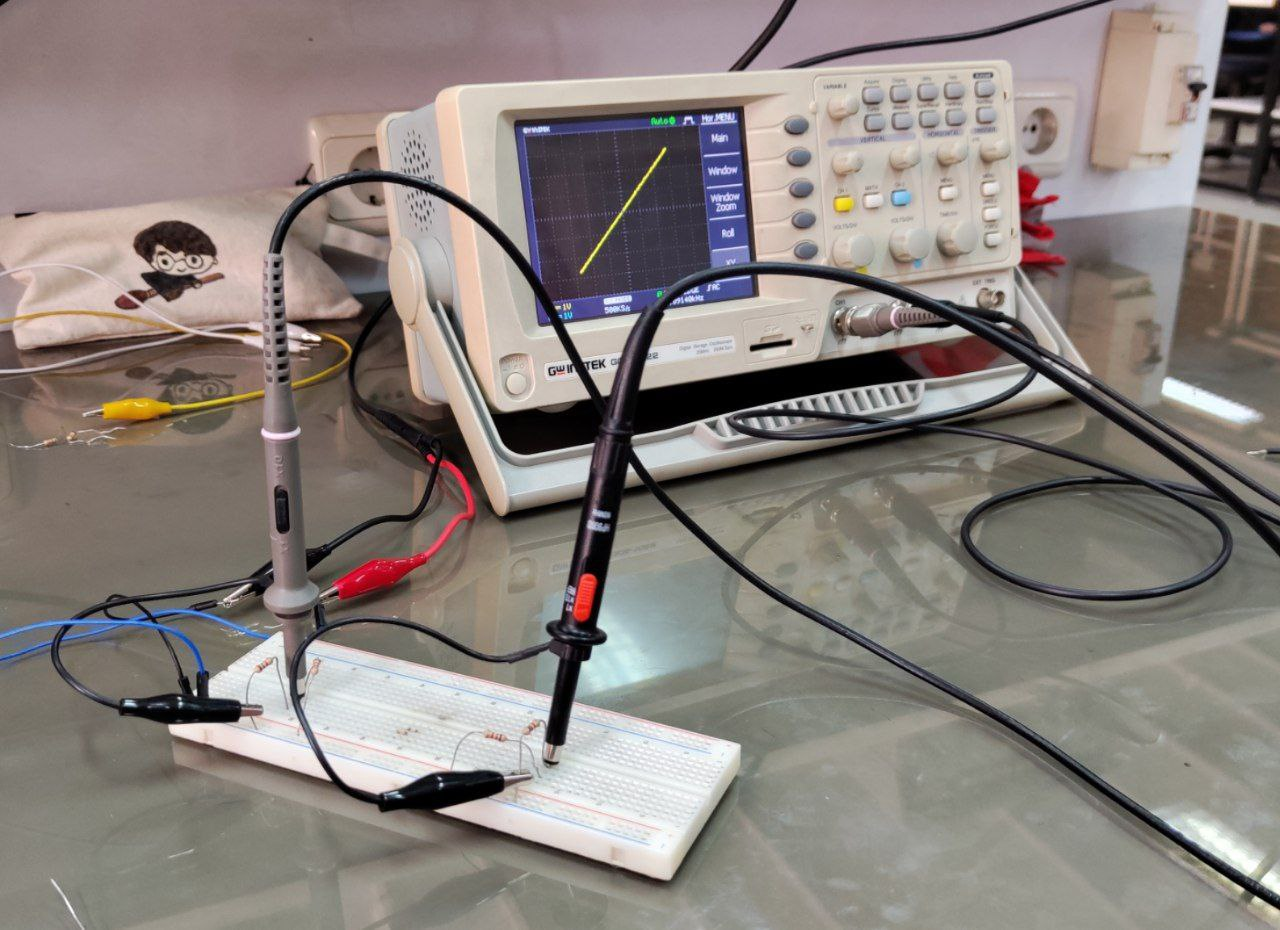
\includegraphics[scale=\PicScale,angle=0]{Fig/1000.jpeg}
                \caption{A photo of all the setup and I don't have any idea why should i put it here just because my friend i guess said and I don't know whatever I don't care about my life anymore and I wish I die as soon as possible and also it doesn't mean that I don't trust him I just didn't think at the first that putting photos makes any sense otherwise his comments and ideas are wonderful Edit: now I saw that this photo is very cute and I took a perfect photo which meets high standards just look at the fancy background of this masterpease(I donno the right spell of that word) and how that beautiful Harry Potter pencil case matches the rest of setup and the position of probes and the color difference between them and the perfect line on the screen which I prefer diode characteristic curve because it's more complicated and matches with Electrical engineering.}
            \end{figure}
            \begin{figure}[H]
                \centering
                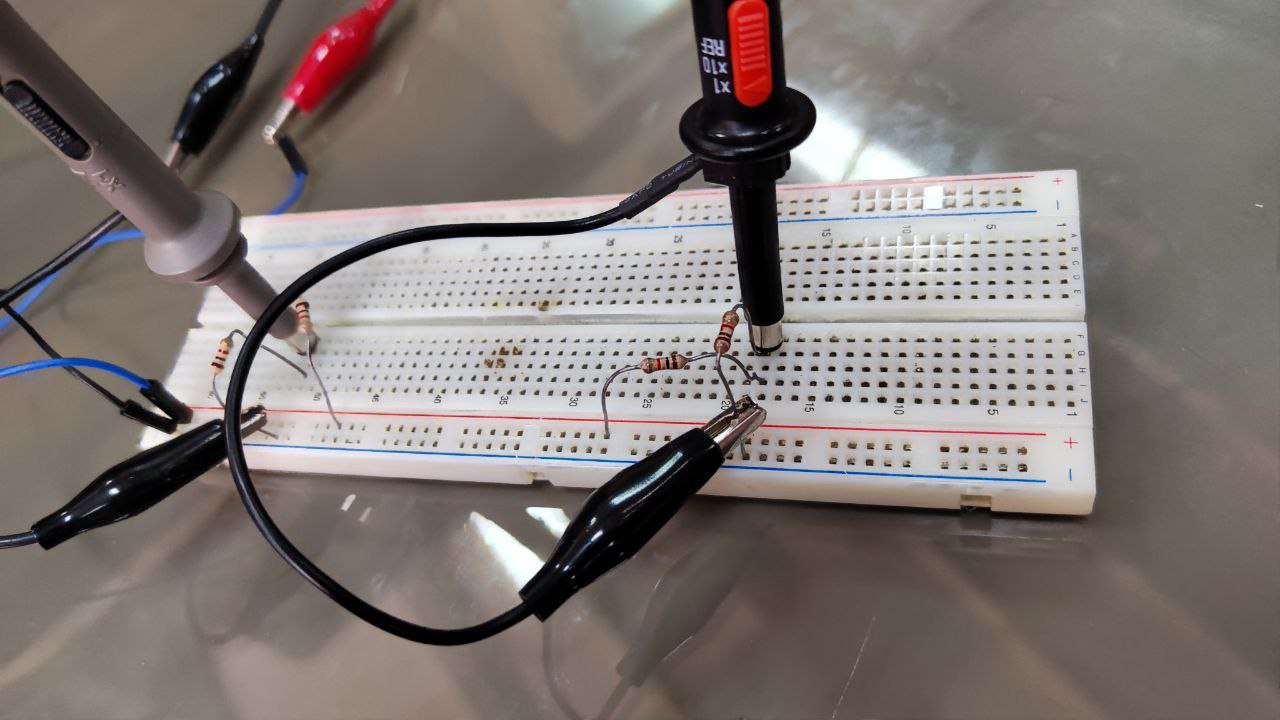
\includegraphics[scale=\PicScale,angle=0]{Fig/40.jpeg}
                \caption{The circuit.}
            \end{figure}
            \begin{figure}[H]
                \centering
                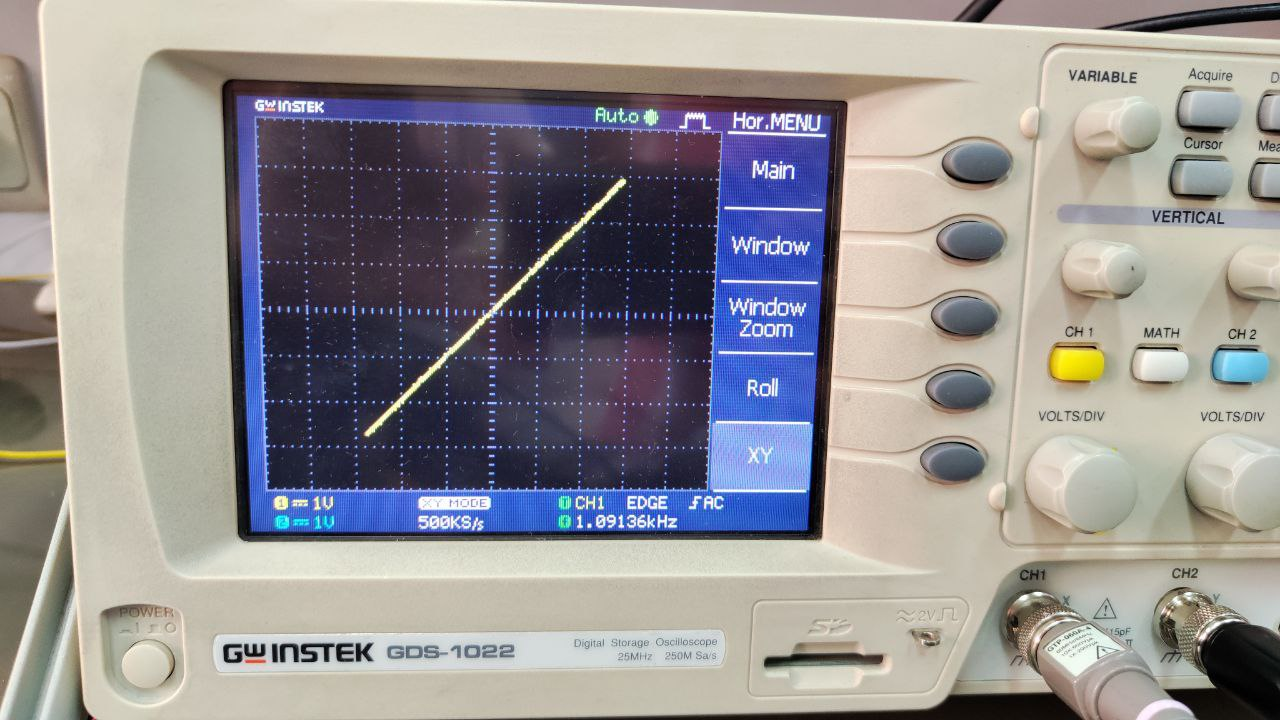
\includegraphics[scale=\PicScale,angle=0]{Fig/41.jpeg}
                \caption{The oscilloscope showing resistor characteristic curve.}
            \end{figure}
        }
    \end{subquestion}

    %--------------------------------------------
    \begin{subquestion}{Repeat the previous part for a diode.}
        \answer{
            \begin{figure}[H]
                \centering
                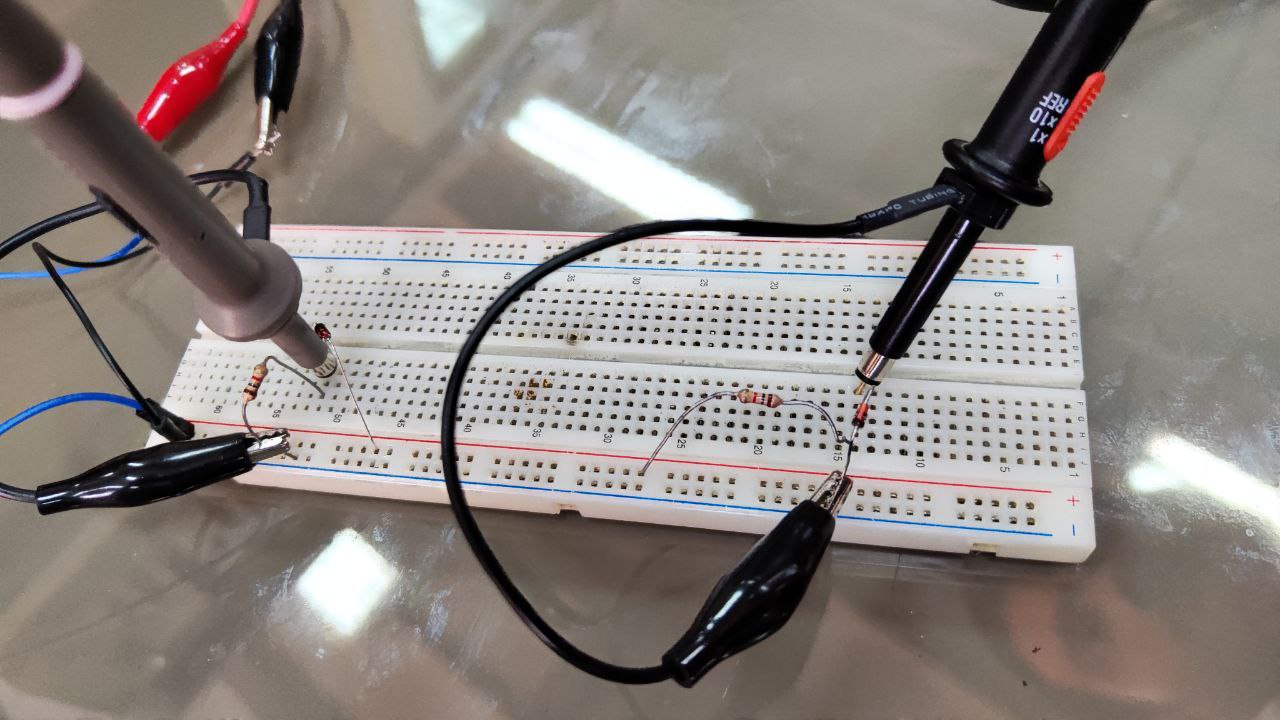
\includegraphics[scale=\PicScale,angle=0]{Fig/42.jpeg}
                \caption{The circuit.}
            \end{figure}
            \begin{figure}[H]
                \centering
                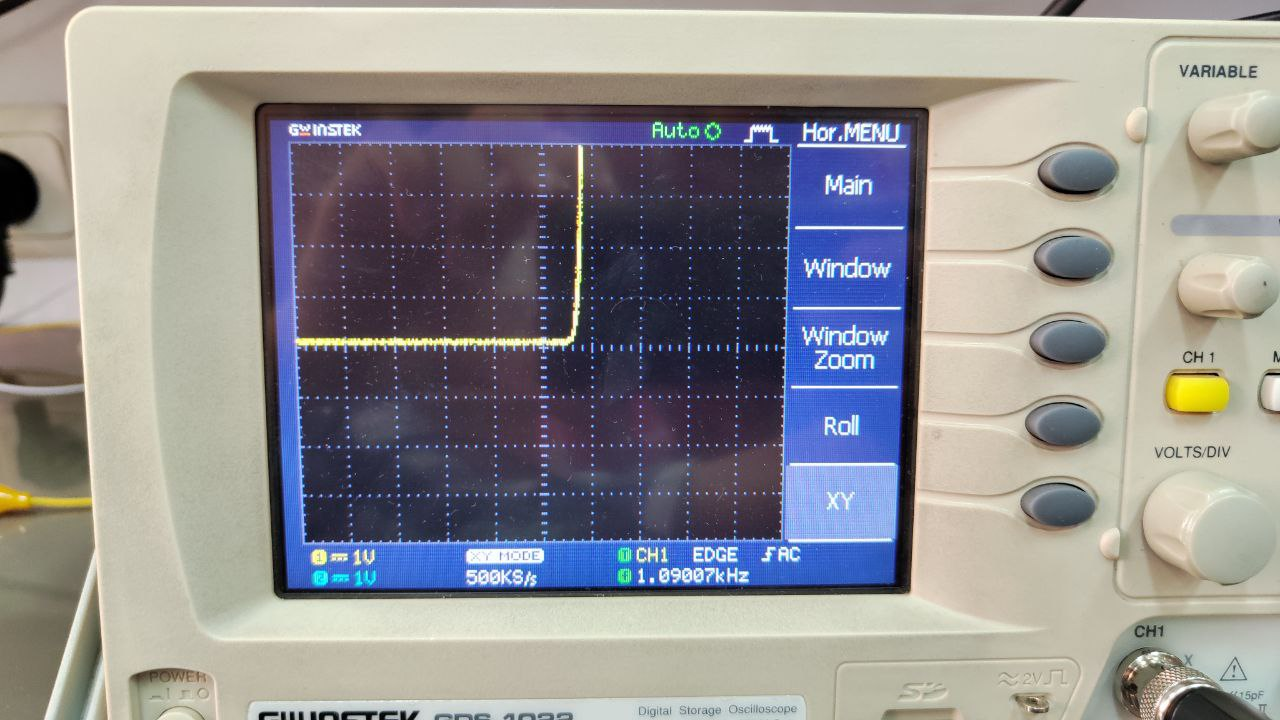
\includegraphics[scale=\PicScale,angle=0]{Fig/43.jpeg}
                \caption{The oscilloscope showing diode characteristic curve.}
            \end{figure}
        }
    \end{subquestion}


\end{question}

%----------------------------------------------------------------------------------------
%	QUESTION 1
%----------------------------------------------------------------------------------------

\begin{question}

    \questiontext{Consider the real capacitor modeled in Fig. \ref{fig:cir4}. }

    \begin{figure}[H]
        \centering
        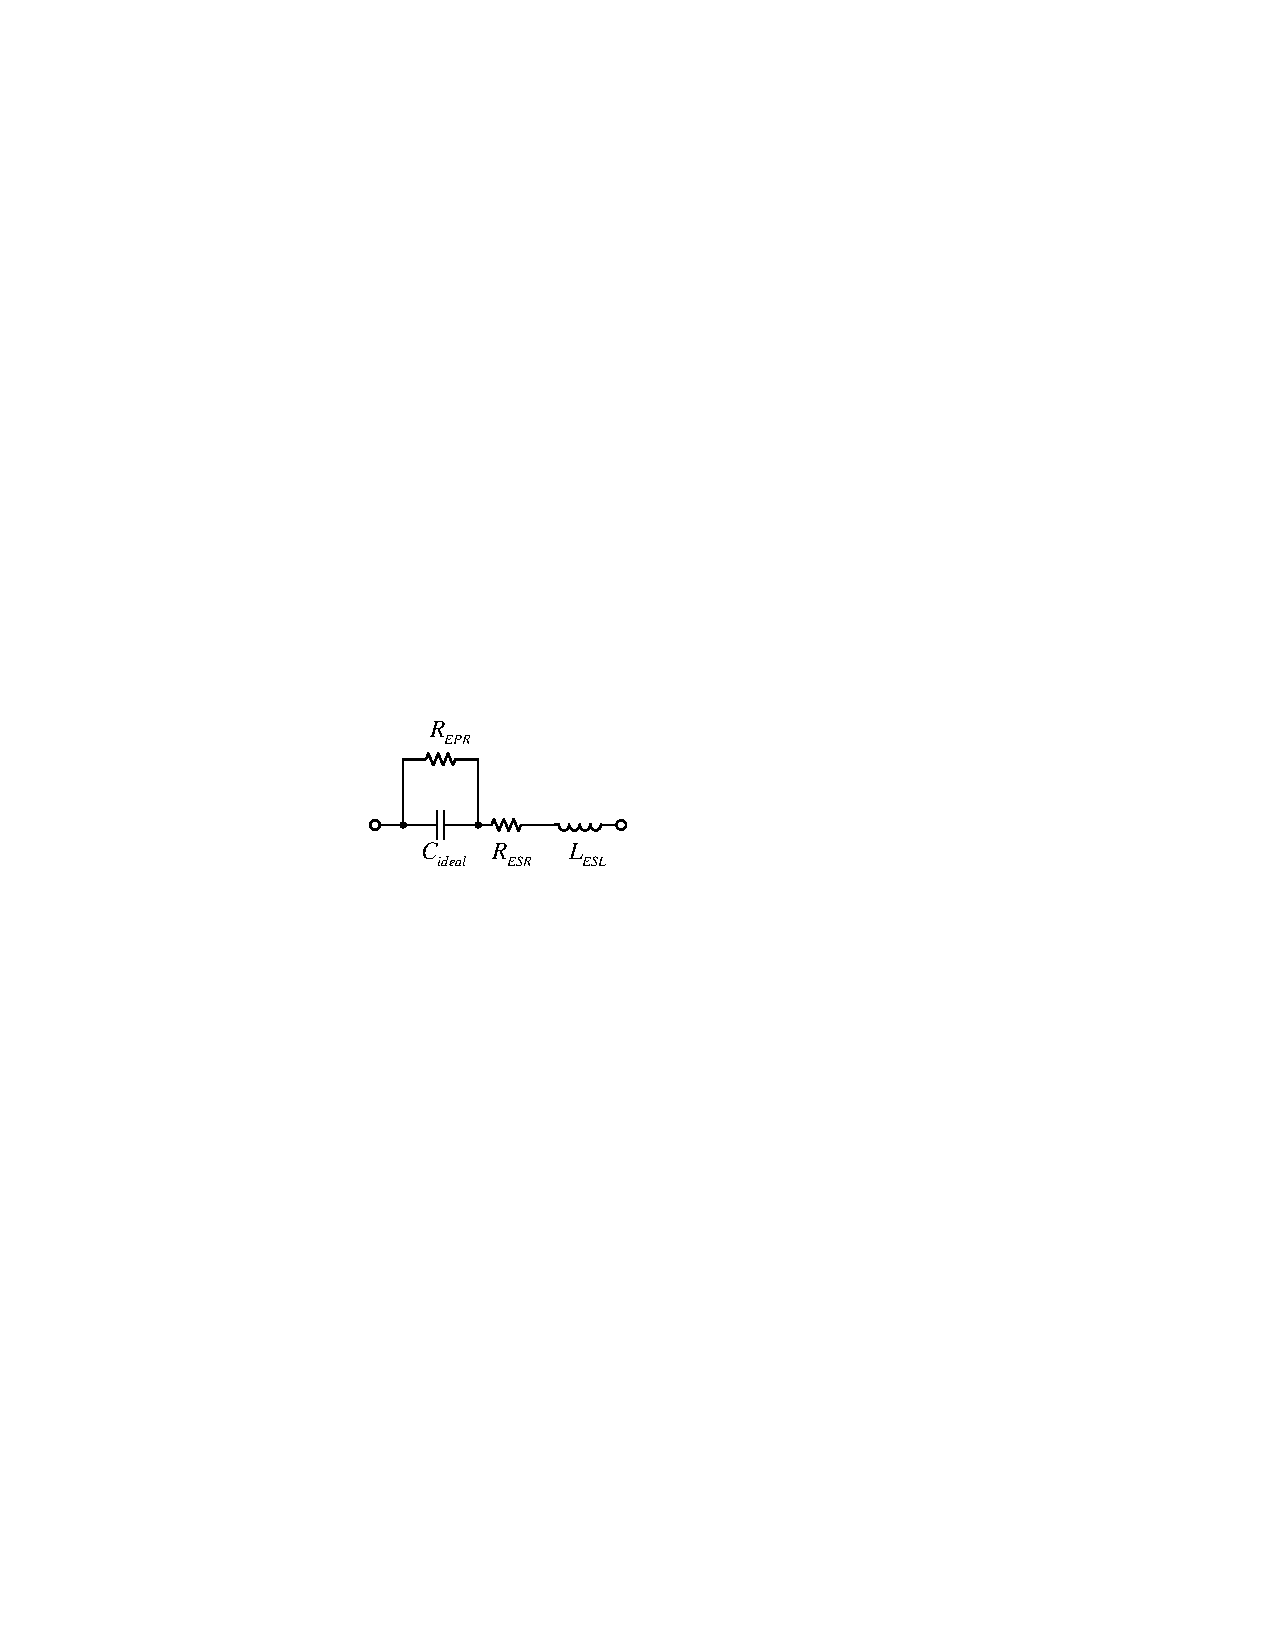
\includegraphics[scale=1.5,angle=0]{Fig/cir4.pdf}
        \caption{Real capacitor model.} \label{fig:cir4}
    \end{figure}

    %--------------------------------------------
    \begin{subquestion}{Assume that the sinusoidal voltage $v_C(t)=A\cos(\omega t+\theta)$ is applied to the capacitor. Find the corresponding capacitor current $i_C(t)$ for ideal values of $R_{EPR}$, $R_{ESR}$, and $L_{ESL}$ and show that it has sinusoidal form.}
        \answer{}
    \end{subquestion}

    %--------------------------------------------
    \begin{subquestion}{Use PSpice AC sweep analysis to plot the amplitude and phase of the capacitor current versus $f=\frac{\omega}{2\pi}$ when the capacitor voltage is $v_C(t)=\cos(\omega t+\theta)$ and $R_{EPR}$, $R_{ESR}$, and $L_{ESL}$ have ideal values.}
        \answer{}
    \end{subquestion}

    %--------------------------------------------
    \begin{subquestion}{Use PSpice parametric analysis to plot the amplitude and phase of the capacitor current versus $f=\frac{\omega}{2\pi}$ for the capacitor voltage $v_C(t)=\cos(\omega t+\theta)$ and different suitably selected values of $R_{EPR}$, $R_{ESR}$, and $L_{ESL}$. Discuss how the parasitic parameters $R_{EPR}$, $R_{ESR}$, and $L_{ESL}$ affect the performance of the capacitor. }
        \answer{}
    \end{subquestion}

\end{question}

\assignmentSection{Bonus Experiments}

%----------------------------------------------------------------------------------------
%	QUESTION 8
%----------------------------------------------------------------------------------------
\begin{question}

    \questiontext{Write a MATLAB/Python code to plot the Lissajous curve corresponding to the voltage signals $v_x(t)=A_x\cos(\omega_x t+\theta_x)$ and $v_y(t)=A_y\cos(\omega_y t+\theta_y)$.
    }

    %--------------------------------------------
    \begin{subquestion}{Use the developed code to plot sample Lissajous curves for various values of $A_x$, $A_y$, $\omega_x$, $\omega_y$, $\theta_x$, and $\theta_y$. }
        \answer{}
    \end{subquestion}

    %--------------------------------------------
    \begin{subquestion}{Assume that $\frac{\omega_x}{\omega_y}=\frac{m}{n}$, where $\frac{m}{n}$ is a fractional number. Discuss how the ratio $\frac{\omega_x}{\omega_y}$ can be found from the corresponding Lissajous curve?}
        \answer{}
    \end{subquestion}

\end{question}


%----------------------------------------------------------------------------------------
%	QUESTION 10
%----------------------------------------------------------------------------------------

\begin{question}

    \questiontext{Return your work report by filling the \LaTeX template of the manual. Include useful and high-quality images to make the report more readable and understandable.}

\end{question}

%----------------------------------------------------------------------------------------

\end{document}
